% PROjet d'enseignement

% Détails responsabilités filière

%   20% 

% Motivations pour l'enseignement

% 3 lettres reco
% copie des contrats

\documentclass[11pt]{article}
%\usepackage{makeidx}
%\usepackage{graphicx}
\usepackage[utf8]{inputenc}
\usepackage[OT1]{fontenc}
\usepackage[francais]{babel}
%\usepackage{a4wide}
\usepackage{fancybox}
%\usepackage{hyperref}
\usepackage{comment}
\usepackage{geometry}
\usepackage{eurosym}
\usepackage{amssymb}
\usepackage[pdftex]{graphicx}
\usepackage{pdfpages}
\usepackage{here}

\usepackage{pgf}
\usepackage{pdfswitch}
\hypersetup{urlcolor=black,linkcolor=black,citecolor=black} % Keep printer friendly
%\geometry{hmargin=3.5cm, bottom=22mm,vmargin=2.5cm }
\geometry{top=23mm,bottom=27mm,left=17mm,right=27mm,headsep=0pt}
\setlength{\parindent}{1cm}


\usepackage[twoside,citeonce(page)]{footbib}
\usepackage{todonotes}
\usepackage{sectsty}

\footbibliography{generalbiblio}
\footbibliographystyle{plain}

\newcommand {\burl}[1]{\url{http://icps.u-strasbg.fr/~genaud/courses/#1}}

\newcommand {\rubrique}[1]{
\begin{flushleft}
{\large\bf #1}
\rule{\linewidth}{1mm}
\end{flushleft}
}
\newcommand{\pmpi}{\mbox{\textsc{P2P-MPI}}}


\makeatletter
\def\thebibliography#1{\subsection*{\rule{\linewidth}{1pt}\@mkboth
%\def\thebibliography#1{\subsection*{\rubrique{\large\bf Références biliographiques}\@mkboth
  {PUBLICATIONS}{PUBLICATIONS}}\list
      {[\arabic{enumi}]}{\settowidth\labelwidth{[#1]}\leftmargin\labelwidth
      \advance\leftmargin\labelsep
      \usecounter{enumi}}
      \def\newblock{\hskip .11em plus .33em minus .07em}
      \sloppy\clubpenalty4000\widowpenalty4000
      \sfcode`\.=1000\relax}
    \makeatother


\begin{document}
%------------------------- Page de Garde -------------------
%\setlength{\parskip}{0mm}
\thispagestyle{empty}
\vspace*{\stretch{1}}




\rule{\linewidth}{1mm}
\begin{center}
\Large{\textbf{Dossier de Candidature\\
aux fonctions de \\
Professeur des Universités\\
Poste 4019 --- ENSIIE - Antenne de Strasbourg}}\\[5mm]
\Large{Stéphane \textsc{Genaud}}\\[1cm]

\rule{\linewidth}{1mm}
\vspace*{\stretch{2}}\\
\vspace{3cm}
%\DeclareGraphicsExtensions{.jpg}
%\includegraphics[width=5cm]{inria.jpg}
\end{center}
\begin{center}
Date: \today\\
\end{center}

\newpage
\mbox{}%blank page 

\setlength{\parindent}{5mm} %% restore a decnt value
\setlength{\parindent}{0mm}
%\setlength{\itemsep}{1mm}
\newpage


\begin{center}
\huge{\textsc{Table des matières}}
\end{center}
\vspace{2cm}


\tableofcontents

\noindent
%\rule{\linewidth}{0.3mm}


\newpage
% Sections' styles

%save
\newcommand{\mysf}{\sectionfont}
\sectionfont{\sectionrule{3ex}{0pt}{-1ex}{2pt}}
\subsectionfont{\sectionrule{1ex}{0pt}{-1ex}{1pt}}

%-------- C V -----------------------------------

\section{Curriculum Vit{\ae}}

\setlength{\tabcolsep}{5pt}

\subsection{\'Etat civil}

\medskip

\noindent
\begin{tabular}{llp{\linewidth}}

				%& \rule{\linewidth}{.2mm} \\
\hspace{1cm}	& Prénom et nom :			&\textbf{Stéphane GENAUD}\\
		 	& Date et lieu de naissance :	& Né le 10 mars 1969 à Forbach (57).\\
			& Nationalité :			& Française. \\
			& Situation familiale :		& Marié, 2 enfants. \\
			& Adresse professionnelle :	& ENSIIE, 1 r. Cassini,\\
			&      				& F-67400 Illkirch\\
			&				& Tél. : +33 (0)3 69 200 231\\ 
			& Adresse électronique :	& \texttt{genaud@ensiie.fr}\\
			& Page personnelle :		& \texttt{{\url{http://icube-icps.unistra.fr/index.php/Stéphane_Genaud}}}\\[5mm]
				%& \rule{\linewidth}{.2mm} \\

\end{tabular}

%---------------------- P O S I T I O N   A D M I N I S T R A T I V E ------------------------------
\vspace{8mm}
\textbf{\underline{Position administrative actuelle}}
\vspace{5mm}

\begin{itemize}
\item Fonction :\textbf{Directeur de l'antenne de Strasbourg de l'ENSIIE} (depuis mars 2013).\\[1mm]
       
\item Position administrative  (depuis novembre 2012): 
   \begin{itemize}
	\item[$\rhd$] Maître  de conférences mis  à disposition de  l'ENSIIE par
          l'Université de Strasbourg (UdS),
	\item[$\rhd$] Chercheur  au Laboratoire des sciences  de l'ingénieur, de
          l'informatique et de l'imagerie (\textsc{Icube},  UMR 7357 CNRS-UdS), membre de
          l'équipe \textit{Image et Calcul Parallèle Scientifique} (ICPS).\\
   \end{itemize}

\item Titulaire de la \textbf{Prime d'Excellence Scientifique} depuis septembre 2009.\\

\item \textbf{Qualifié aux fonctions de Professeur des Universités} dans la 
              section 27 en 2010.\\
	\indent {\small Numéro de qualification~:~PR-2010-27-10127207589}\\[2mm]
\end{itemize}


%---------------------- F O R M A T I O N   U N I V E R S I T A I R E ------------------------------

\subsection{Formation Universitaire}
\medskip
\noindent
\begin{tabular}{lp{14.8cm}}
		%		& \rule{\linewidth}{.2mm} \\
	\textbf{2009} &  \textbf{Habilitation à diriger des recherches} en informatique \\
			  &	Université Henri Poincaré, Nancy. \textit{Soutenue le 8/12/2009}\\
      		  &	Titre du mémoire : {\em Exécutions de programmes parallèles à passage de messages sur grille de calcul}.\\
			  &	Jury~: 
				\begin{small}
				\begin{itemize}
				\item Pascal Bouvry (PU, Université du Luxembourg), Examinateur,
				\item Christophe Cérin (PU, Université Paris 13), Rapporteur,
				\item Frédéric Desprez (DR, INRIA Grenoble Rhônes-Alpes), Rapporteur,
				\item Claude Godart, (PU, Université Henri Poincaré), Président,
				\item Jens Gustedt (DR, INRIA Nancy Grand-Est), Garant,
				\item Thierry Priol (DR, INRIA Rennes Bretagne-Atlantique), Rapporteur.
				\end{itemize}
				\end{small}\\[2mm]
	

	\textbf{1997} & \textbf{Doctorat en Sciences, mention Informatique}\\
			  & Université Louis Pasteur, Strasbourg.\\
      		  & Titre du mémoire: {\em Transformations de programmes \textsc{Pei} : applications au parallélisme de données}.\\
		        & Jury~:
				\begin{small}
				\begin{itemize}
					\item Luc Bougé (PU, \'{E}NS Lyon), Rapporteur,
			    		\item Christian Lengauer (PU, Université Passau, Allemagne), Examinateur,
					\item Catherine Mongenet (PU, Université Louis Pasteur), Rapporteur interne,
					\item Guy-René Perrin (PU, Université Louis Pasteur), Directeur de thèse,
					\item Patrice Quinton (PU, Université de Rennes 1), Rapporteur.
				\end{itemize}
				\end{small}\\[2mm]
	\textbf{1993} &  \textbf{Diplôme d'\'{E}tudes Supérieures Spécialisées} (DESS) en Informatique du parallélisme, 
				  Université de Franche-Comté, Besançon. Mention {\em très bien} (major).\\[2mm]
	\textbf{1991} &  \textbf{Bachelor of Sciences} (BSc) in European Informatics, Sheffield Hallam University.\\[2mm]
%	\textbf{1989} &  {\bf Diplôme Universitaire de Technologie (DUT)} en informatique, Institut Universitaire de 
%					Technologies de Nantes, Université de Nantes.\\[5mm]
%		%	& \rule{\linewidth}{.2mm} \\

\end{tabular}
%\newpage


\subsection{Expérience professionnelle}

\noindent
\begin{tabular}{p{2cm}p{14.3cm}}
%		& \rule{\linewidth}{.2mm} \\
% 	depuis sept. 2009 &  \textbf{Maître de conférences en Informatique} à l'Université de Strasbourg (UdS):\\[-7mm]
%		&\parbox[t]{13.7cm}{%
%            \begin{itemize}
%				  \item[$\rhd$] Enseignant à l'\'Ecole de Management Strasbourg,
%				  \item[$\rhd$] Chercheur au Laboratoire des Sciences de l'Image, de l'Informatique et de la Télédétection (LSIIT, UMR 7005 CNRS-UdS),
%équipe \textit{Image et Calcul Parallèle Scientifique} (ICPS).
%				\end{itemize}
%				\vspace{3mm}
% 				}\\

 	 \textbf{2013--~~~}  &  \textbf{Directeur de l'antenne de Strasbourg de l'ENSIIE}\\
	 \textbf{2009--2012}  &  \textbf{Maître de conférences en Informatique} à l'Université de Strasbourg\\[2mm]
 	 \textbf{2007--2009}  &  \textbf{Détaché Chargé de Recherche} au Laboratoire Lorrain de Recherche en Informatique et ses Applications
(LORIA, UMR 7503 CNRS-INPL-INRIA-UHP-Nancy 2), équipe projet INRIA \textsc{AlGorille}.\\[2mm]

	\textbf{1998--2007}    &  \textbf{Maître de conférences en Informatique} à l'Université Robert Schuman, Strasbourg:\\[-3mm]
				&\parbox[t]{13.7cm}{%
                          \begin{itemize}
				  \item[$\rhd$] Enseignant à l'IECS, Université Robert Schuman,
				  \item[$\rhd$] Chercheur au LSIIT, UMR 7005 CNRS-ULP, équipe ICPS.
				\end{itemize}
				\vspace{3mm}
 				}\\


	\textbf{1996--1998} &  \textbf{Attaché Temporaire d'Enseignement et de Recherche} au département d'informatique 
de l'IUT de l'université Robert Schuman.\\[2mm]
	\textbf{1993--1996} & Doctorant à l'Université de Franche-Comté, Besançon, puis Université Louis Pasteur, Strasbourg. Directeur de thèse: Guy-René Perrin.\\[2mm]
\end{tabular}


%------------------ R E S P O N S A B I L I T E S ---------------------------

\subsection{Responsabilités principales}
\vspace{3mm}
\medskip

\begin{itemize}
\item
 	\textbf{Responsabilités pédagogiques}\\[-1mm]
	\begin{itemize}
		\item \textbf{Directeur de l'antenne de Strasbourg de l'ENSIIE}, depuis 03/2013.
		\item Directeur délégué aux Systèmes d'Information de 
		      l'\'Ecole de Management Strasbourg 07/2011-09/2012.
		\item Responsable de la filière \textit{Système d'Information} 
		      du master Management International de l'IECS de 2002 à 2007.\\
	\end{itemize}

 	\textbf{Responsabilités recherche}
	\begin{itemize}
		\item Responsable du thème de recherche \textit{Grilles} dans 
		      l'équipe ICPS du LSIIT de 2001 à 2007. 
			Reprise du thème à mon retour dans l'équipe en septembre 2009.
		\item Membre du conseil scientifique du département \emph{Expertise 
		      pour la recherche de l'UdS} depuis 2010.\\
	\end{itemize}

 	\textbf{Responsabilités administratives et collectives}
	\begin{itemize}
		\item Membre de 3 commissions de spécialistes entre 2004 et 2008.
		\item Membre du comité d'experts UdS (section 27) depuis 2009 et 
		      membre dans 2 comités de sélection externes.
	      \item Co-responsable des systèmes d'information de mon 
		      établissement depuis 2001.\\
	\end{itemize}
\end{itemize}


%---------------------------- E N J E U ------- --------------------------------
\newpage
\setlength{\parindent}{5mm}
\setlength{\itemsep}{2mm}
%\sectionfont{\mysf}

\section{L'enjeu du poste}

\medskip
\emph{Ce  premier  poste permanent  ouvert  par  l'ENSIIE  à Strasbourg  a  pour
  objectif la \textbf{pérennisation} de l'antenne. Cette section a pour objectif
  de montrer  mon analyse de la  situation et des  défis à relever pour  mener à
  bien le projet.}\\

Après une  phase de démarrage réussie,  de la rentrée  2009 à 2013, le  relai de
croissance doit maintenant être trouvé  pour assurer un fonctionnement normal de
l'antenne.   La phase  de démarrage  menée par  Pierre Tellier,  a nécessité  un
travail considérable  pour assurer à  la fois le fonctionnement  quotidien usuel
d'une école avec des moyens limités et en même temps faire connaître l'existence
de cette  nouvelle antenne.   Il s'agisssait d'installer  l'école dans  le tissu
économique local  d'une part, et d'accroître  la notoriété de l'école  au niveau
régional et national pour attirer les bons étudiants d'autre part.  Ce démarrage
n'a  également  pu  se  faire  que grâce  a  l'aide  des  collectivités  locales
(communauté urbaine de Strasbourg et région Alsace) ainsi que de l'Université de
Strasbourg. Les collectivités locales aident  l'antenne par une subvention ainsi
que par un  soutien immobilier au projet, tandis que  l'Université de Strasbourg
apporte son  soutien à travers le  corps de ses enseignants-chercheurs  (EC). La
phase  de démarrage  a montré  la faisabilité  et l'intérêt  du projet,  et nous
sommes entrés depuis la dernière rentrée dans une nouvelle phase où il s'agit de
gérer des effectifs étudiants qui font  de l'antenne une école d'ingénieur ayant
une place à part entière sur la région.  C'est une phase délicate, car malgré le
contexte budgétaire difficile, des ressources permanentes devront être dédiées à
l'antenne.   Il  s'agit  donc  d'optimiser  ces  ressources  et  les  moyens  de
développement à disposition  pour parvenir à l'objectif  d'une centaine d'élèves
par promotion sur le moyen terme.\\


Je  distingue quatre  leviers  indispensables  à la  réussite  du projet  ENSIIE
Strasbourg:
\begin{enumerate}
\item la reconnaissance de l'antenne par les entreprises du bassin d'emploi,
\item la reconnaissance de l'antenne par les étudiants au niveau national,
\item la bonne insertion de  l'antenne dans l'écosystème local de l'enseignement
  supérieur et recherche,
\item le financement de l'antenne.
\end{enumerate}


\paragraph{Entreprises} 
Le point 1. est crucial car c'est la demande des entreprises qui est à l'origine
de la création de l'antenne.  Aujourd'hui,  l'école est très bien implantée dans
le  tissu  industriel local  grâce  au  travail  de Pierre  Tellier.   Plusieurs
entreprises ont  dès la création  proposé un soutien  solide sous la  forme d'un
partenariat   (Abase   Europe,   CGI   et   Euro   Information   Développement).
L'organisation  d'évènements  réguliers  a  aussi fait  croître  le  cercle  des
entreprises qui viennent rencontrer les élèves dans nos locaux (la \emph{rentrée
  des  entreprises},  les exposés  thématiques  faits  par les  entreprises,  le
\emph{startup week-end}),  la journée thématique annuelle  (que j'organise cette
année sur le Cloud Computing%
\footnote{\url{http://www.ensiie-developpement-strasbourg.fr/evenements/cloud-computing/}}),
Nous sommes également présents à l'extérieur (la \emph{nuit de l'info}, le forum
AlsaceTech, ...).  Depuis septembre 2012, j'ai  pu opérer la transition dans nos
relations  avec  les entreprises.   L'introduction  d'un  nouveau contact  à  la
direction  de  l'antenne  était  important  car le  projet  en  démarrage  était
fortement personnalisé  par Pierre  Tellier. Les nombreux  évènements extérieurs
auxquels  l'ENSIIE participe,  ainsi que  visites des  nombreux stagiaires,  m'a
permis de rencontrer une grande partie des entreprises cette année écoulée. J'ai
pu égalemet pu initier de nouveaux types de contacts :
\begin{itemize}
\item  Les projets  R\&D  proposés  à partir  de  cette  rentrée permettent  aux
  entreprises de proposer des sujets innovants à un groupe de quatre élèves pour
  une  durée-homme de  150h (valorisé  6 ECTS).   Le projet  est encadré  par un
  permanent de  l'ENSIIE et la conduite  doit suivre une trame  générique à tous
  les projets.

\item  \`A  travers  AlsaceTech,  la  CCI  favorise  la  mise  en  relation  des
  entreprises et des écoles d'ingénieurs.   Nous avons aujourd'hui en permanence
  plusieurs demandes  de réalisations  qui sont redirigées,  selon la  nature du
  travail,  vers des  projets  R\&D  ou vers  la  Junior  Entreprise de  l'ENSIIE
  Strasbourg.

\item L'ENSIIE est aussi sollicitée pour des projets innovants. J'ai par exemple
  répondu récemment à la demande  d'accompagnement d'une startup dans le domaine
  des biotechnologies  afin de jouer  un rôle d'assistance à  maîtrise d'ouvrage
  vis-à-vis de leur prestataire. Cette demande entre dans le cadre du dispositif
  homme-ressource de la région, relayée par Alsace Innovation.

\item Enfin, avec le bureau des élèves, nous avons mis en place un parrainage de
  promotion  propre  à Strasbourg.   Le  parrain  est  une entreprise  qui  peut
  entretenir  des  relations privilégiées  avec  l'école  en contre-partie  d'un
  soutien logistique et financier. 
  

\end{itemize}

\medskip
Ces  contacts  permanents et  denses  avec  le  monde industriel  permettent  de
réaffirmer la volonté de l'école d'être bien ancrée dans son environnement, et de
fournir des cadres de haut niveau aux entreprises.



\paragraph{Étudiants entrants} 
Le point 2. est en passe d'être  réussi. Même si la notoriété requiert un effort
constant de  communication, les recrutements  à cette rentrée de  septembre 2013
montrent  un net  gain d'attractivité  de l'antenne  à la  fois sur  le concours
Centrale-Supélec,  ou  en admission  sur  titre.   L'antenne accueille  à  cette
rentrée 25 élèves issus des CPGE,  contre 12 l'année précédente.  La plupart des
élèves ayant  indiqué ENSIIE  Evry dans  leurs voeux  ont mis  ENSIIE Strasbourg
immédiatement après, et vice-versa, ce qui indique que l'ENSIIE est perçue comme
une seule  et même  école proposant  une formation  équivalente quelque  soit le
site. Les  rangs des derniers intégrés  sont quasiment équivalents sur  les deux
sites.   Concernant  les  candidatures  en   admission  sur  titre,  elles  sont
légèrement plus nombreuses  pour Strasbourg (35) que pour Evry,  et leur origine
géographique s'est étendue à toute la France  pour la première fois, même si une
majorité    provient    de    l'IUT   d'informatique    de    l'Université    de
Strasbourg. L'évolution des effectifs  figure dans la table \ref{tab:effectifs}.
Les efforts que  nous faisons pour continuer d'accroître la  notoriété passe par
les salons  nationaux (l'antenne est  souvent représentée à  travers AlsaceTech)
mais l'action la plus efficace reste la  promotion dans les CPGE par les anciens
élèves   qui   reviennent  présenter   l'école   dans   leur  lycée   d'origine.
Mécaniquement, la notoriété augmente avec le  nombre d'élèves issus des CPGE. Au
plan régional, nos portes ouvertes, notre présence aux Journées des Universités,
et  des   présentations  que  j'ai  faites   dans  les  IUT  de   Strasbourg  et
Belfort-Montbelliard succitent l'intérêt pour une admission sur titre.

\begin{centering}
\begin{table}[hbt]
\begin{center}
\begin{tabular}{|c|c|c|c|c|c|}
\hline
Année &	Total &  Concours & Admission sur  &	Admission sur  & 	Part  \\
      & promotion &  CPGE & titre (France) &     titre (étranger)&     Alsace \\
\hline
% élèves alsaciens
2009/2010	& 9	& 5	& 4	& 0	    & 33\% \\
2010/2011	& 16	& 8	& 4	& 4	    & 31\% \\
2011/2012	& 18	& 6	& 7	& 5	    & 33\% \\
2012/2013	& 30	& 12	& 14	& 4	    & 43\% \\ 
2013/2014	& 40	& 25    & 13	& 2	    & 39\% \\
\hline
\hline
\end{tabular}
\end{center}
\caption{Évolution des effectifs depuis le démarrage de l'antenne.}
\label{tab:effectifs}
\end{table}
\end{centering}


\paragraph{Formation et Recherche}
Le point 3.  est  également un levier fondamental : une  bonne insertion au sein
des formations universitaires  et des laboratoires de  recherche est prioritaire
pour faire de l'école une  ``brique'' indispensable de l'ensemble.  Cette brique
apporte des bénéfices nouveaux:
\begin{itemize}

\item L'existence  de l'antenne  renforce l'attractivité du  site Strasbourgeois
  dans le domaine  de l'informatique. L'ENSIIE attire en effet  des étudiants au
  niveau local  : la formation  représente pour  les meilleurs étudiants  du DUT
  informatique de l'Université de  Strasbourg, une poursuite d'études attractive
  à laquelle  ils souscrivent largement  alors qu'ils partaient  auparavant pour
  rejoindre  d'autres  écoles d'ingénieurs  en  France.   Nous avons  établi  un
  partenariat    privilégié   avec    le    département   informatique    Robert
  Schumann. Depuis  2010, le dispositif  \textit {Passerelle} depuis  permet aux
  cinq meilleurs étudiants  d'entrer à l'ENSIIE Strasbourg. Il a  été convenu de
  faire évoluer  le dispositif  vers une filière  spécificique dans  PostBac qui
  donnerait comme débouché à l'issue du DUT informatique, une poursuite d'études
  dans l'une des deux formations d'ingénieur, \textit{Infrastructures Numériques
    et Objets Communicants} à Télécom  Physique Strasbourg ou celle de l'ENSIIE.
  L'ENSIIE  attire  également au  niveau  national  (61\%  hors Alsace  à  cette
  rentrée),  voire international  (Campus France  + conventions  internationales
  comme  Xidian, issues  du partenariat  Mines-Télécom).  C'est  actuellement la
  seule formation en informatique à Strasbourg avec un rayonnement aussi large.

\item L'ENSIIE  attire des étudiants  à proximité de l'Université,  et l'antenne
  doit s'appuyer sur les  compétences des enseginants-chercheurs de l'Université
  de Strasbourg.  Ceci permet une  mutualisation efficace des enseignements lors
  des semestres 4 et  5 composés à 80\% d'options, et  de manière plus générale,
  favorise la  proximité entre enseignants-chercheurs de  l'Université et élèves
  de l'ENSIIE, nécessaire pour attirer ces élèves vers la recherche.  C'est pour
  cela que nous travaillons actuellement  à une formalisation des relations avec
  l'Université de Strasbourg  sous la forme d'une  association.  Nous souhaitons
  simplifier les  interventions de ECs  de l'Université  à l'ENSIIE. De  même, à
  l'occasion de la nouvelle offre quinquénnale de l'Université, j'ai retravaillé
  et renouvellé  les conventions  passées avec les  Masters en  informatique ISI
  (Informatique et Sciences de l'Image) et RISE (Réseau Informatique et systèmes
  Embarquées) qui  permettent aux  élèves de  l'ENSIIE ayant  suivi suffisamment
  d'options d'obtenir l'un de ces  masters en double-cursus. Les contraintes ont
  ainsi été  simplifiées pour  encourager les  élèves à souscrire  à ce  type de
  parcours  plus  spécialisé et  orienté  recherche.   En contre-partie  de  ces
  formations ouvertes pour  l'ENSIIE, L'ENSIIE peut également être  un soutien à
  des formations de l'Université, comme dans  le projet de création d'un nouveau
  diplôme d'ingénieur \textit{Infrastructures Numériques et Objets Communicants}
  porté  par Télécom  Physique Strasbourg,  pour lequel  l'ENSIIE assurerait  la
  première année d'enseignement.

\item  Concernant la  recherche,  la présence  des EC  de  l'Université dans  la
  formation  amène davantage  d'élèves à  faire  des stages  recherche dans  les
  équipes de Icube ou de l'IRMA  avec des poursuites éventuelles en thèse.  Deux
  étudiants (dont un  provenant d'Evry ont déjà entamé une  thèse à l'Université
  de  Strasbourg). Plus  d'une  dizaine de  stages  ont déjà  eu  lieu dans  les
  laboratoires de l'Université. 


\end{itemize}

La bonne connaissance  des thèmes de recherche et des  chercheurs à l'Université
est  donc  indispensable  au  directeur  de  l'ENSIIE  Strasbourg  pour  insérer
correctement  l'école  dans cet  environnement.   Le  fléchage  de ce  poste  en
informatique pour le laboratoire Icube va exactement dans ce sens.


\paragraph{Financement}
Le projet  a été démarré à  une période où les  restrictions budgétaires étaient
beaucoup moins  prégnantes qu'aujourd'hui.  Le financement  reste aujourd'hui la
difficulté principale car le Ministère n'a pas pris en compte l'augmentation des
effectifs et des coûts depuis 2009. Ainsi la dotation récurrente et le nombre de
postes  sont  restés  constants  depuis   quatre  ans.   L'aide  financière  des
collectivités locales (et celle  financièrement indirecte de l'Université) était
indispensable à la  phase de démarrage du projet. Cette  subvention s'arrête fin
2014, et nous avons entamé des  négociations avec les collectivités locales pour
que  l'aide financière  puisse être  reconduite sur  2015.  Ceci  permettrait au
directeur de l'ENSIIE  de construire un budget en équilibre  pour 2015, dernière
année avant le nouveau plan quinquennal  démarrant en 2016. Dans ce nouveau plan
quinquennal, le Ministère devra ternir compte du taux d'encadrement relativement
faible  de l'ENSIIE  (1  EC pour  17  élèves) et  acter  l'existence pérenne  de
l'antenne de Strasbourg, qui représentera (en limitant les effectifs à 40 élèves
par  an),  25\%  des  effectifs  d'Evry.  Pour  l'instant,  obtenir  l'aide  des
collectivités locales et de l'Université  nécessite d'entretenir une relation de
confiance,  et de  convaincre  que le  projet  de l'ENSIIE  va  bien amener  une
plus-value aux acteurs locaux, entreprises ou Université.\\



\bigskip
\paragraph{Conclusion}
\emph{A travers ces  quatres volets, j'ai montré les difficultés  mais aussi les
  réussites constatées,  et j'ai esquissé  les actions  que j'étais en  train de
  mener.  Le  reste du dossier  a pour objectif de  me présenter en  détails. Il
  montre mon expérience de l'environnement  de l'enseignement supérieur et de la
  recherche à Strasbourg, qui est à mon sens, un atout pour réussir le projet de
  l'antenne ENSIIE de Strasbourg.}
  





%-------------------------------- E N S G N T  ---------------------------------------------
\newpage

\section{Activités et charges afférentes à l'enseignement}
\label{sc:ensgnt-univ}

\subsection{Activité d'enseignement}

\paragraph{Dans le cadre de ma fonction actuelle}

J'assure cette année  une demi-charge de service d'enseignement  à l'ENSIIE, qui
se  traduit par  l'enseignement  de trois  modules du  tronc  commun :  Systèmes
Informatiques aux semestres 1 et 2, et Middleware au semestre 3. Ce contact avec
les élèves en tant qu'enseignant est pour moi indispensable pour bien comprendre
la dynamique de la promotion.  Ma fonction actuelle de directeur étant largement
consacrée à  gérer le  corps professoral  qui intervient  auprès des  élèves, ce
contact permanent  avec l'enseignement me  permet d'anticiper ou  comprendre les
problèmes qui peuvent se poser au quotidien, d'avoir un avis consultatif sur les
orientations  pédagogiques prises par la direction de la formation pédagogique, 
et de participer à tous les jurys.\\

Cependant, ma  vocation d'enseigner  va au-delà de  l'ENSIIE. J'ai  conservé des
interventions dans d'autres  composantes : cette année,  j'interviendrai dans un
Master  Informatique  de  l'UFR   Mathématique-Informatique  à  l'Université  de
Strasbourg, dans la filière informatique de Télécom Physique Strasbourg, et dans
un cours  d'informatique à Supélec  Campus de  Metz.  Si ces  interventions sont
minimes en terme de volume horaire, ce sont autant d'occasions de rencontrer ces
étudiants et de comprendre  ce qui motive et a motivé  leur orientation. Tout au
long de  ma carrière,  j'ai favorisé ces  expériences d'enseignement  variées, à
différents types  de publics.   Les enseignements  auxquels j'ai  participé sont
listés dans le tableau~\ref{sc:tab-ens}, page~\pageref{sc:tab-ens}.





\paragraph{Activité antérieure}

J'ai été recruté en septembre 1998 sur un poste de maître de conférences 
en informatique (27$^e$ section) dans une composante de l'Université, l'IECS%
\footnote{Institut d'Enseignement  Commercial Supérieur, devenue en  2007, après
  fusion        avec        l'IAE,         l'\'Ecole        de        Management
  Strasbourg. \url{http://www.em-strasbourg.eu/}} dédiée aux sciences de gestion
(6$^e$ section).  Ce  poste préexistant marquait la volonté de  la composante de
développer les  enseignements en systèmes  d'information. \`A mon  arrivée, j'ai
pris en  charge les cours définis  qui avaient trait à  l'informatique.  Puis en
2001,  j'ai  pris  \textbf{la  responsabilité de  la  filière}  \textit{systèmes
  d'information} pour  y développer  et organiser  les enseignements.   Mon rôle
était de définir  et de coordonner les enseignements de  la filière, nécessitant
en plus  des enseignants permanents, de  recruter une dizaine de  vacataires par
an, professionnels de l'industrie dans leur très grande majorité.  D'autre part,
il m'incombait le suivi  des étudiants au travers de la  définition de sujets de
mémoires  de  fin d'études,  la  validation  de  leur  cursus à  l'étranger,  et
l'information  vis-à-vis des  débouchés  professionnels (réunions  d'information
avec des professionnels,  animation d'échanges avec des anciens  de la filière).
Cette activité  s'est arrêtée  en 2007  lorsque je suis  parti en  détachement à
l'INRIA.\\

De retour de détachement, j'ai réintégré  mon poste tout en effectuant plus d'un
tiers de mon  service à l'extérieur de l'établissement  (procédure facilitée par
la  fusion  des  universités  strasbourgeoises), à  l'UFR  de  mathématiques  et
informatique, et à l'ENSIIE qui venait d'ouvrir l'antenne de Strasbourg.


\subsection{Principales charges d'intérêt collectif}

\begin{itemize}
\item[$\bullet$] Directeur délégué aux système d'information à l'EM Strasbourg (sept 2011--).\\
En charge d'un service de trois analystes-programmeurs. Mon rôle au sein de la direction
est de proposer des choix stratégiques pour les services à développer ou acquérir en matière 
de système d'information. Je planifie également la ré-organisation des services existants de 
l'établissment. Ces développements se font en concertation avec l'Université (Direction des 
Usages Numériques et Direction Informatique). Parmi les projets les plus importants~: 
implantation d'un CRM, gestion du processus de recrutement des vacataires, gestion des
étudiants à l'étranger.\\
		

\item[$\bullet$] Responsable de la filière d'enseignement \emph{système d'information} à l'IECS, Strasbourg (2001--2007).\\

\item[$\bullet$] 
Responsable de la mise en place de l'intranet de l'IECS (2000--2003). 
Participation au développement, essentiellement assuré par Christos Karacostas,
pour lequel j'étais l'encadrant de son mémoire de cycle C du CNAM (soutenu en juin 2001).\\

\item[$\bullet$] \textbf{Commissions de spécialistes} section CNU 27:
	\begin{itemize}
		\item titulaire à l'Université Louis Pasteur, Strasbourg, 2004--2008,
		\item suppléant à l'Université de Franche-Comté, Besançon, 2005--2008,
		\item suppléant à l'Université Henri Poincaré, Nancy, 2006--2008.\\
	\end{itemize}
	\item 2010-- : Membre du \textbf{comité d'experts} (9 membres) pour la section 
		27 de l'Université de Strasbourg.
	\item Membre des comités de sélection:
	\begin{itemize}
		\item poste MC 210 UdS Réseaux et Protocole, 2010,
		\item poste MC 1207 Université de Franche-Comté, IUT Belfort Montbéliard, 2010.\\
	\end{itemize}


\item[$\bullet$] 
Participation à l'animation de la communauté des enseignants-chercheurs en informatique, à travers 
l'action collective de l'association SPECIF (Société des Personnels Enseignants et Chercheurs 
en Informatique de France), depuis 2008. Je suis membre du conseil d'administration de SPECIF depuis 
2010. SPECIF est devenue la SIF (Société Informatique de France) depuis le 31/mai/2012.\\

\item[$\bullet$] 
Membre élu, collège A, du conseil scientifique de l'ENSIIE depuis juin 2012. 
\vspace{1cm}
\end{itemize}



%--------------- T A B   E N S E I G N E M E N T S ------------------------------------
\newpage

\begin{table}[H]
\caption{Liste des enseignements}
\begin{center}
{\footnotesize
\noindent \begin{tabular}{|c|c|p{6cm}|c|c|c|c|} \hline &&&&&\\[-8pt]

Année & Filière & Matière & cours & TD & TP &  occurrences \\[5pt] \hline
%&&&&&\\[-8pt]
 
\hline
09-14 (4)
	& Master 2 info		& Applications distribuées, parallélisme et grilles	&  12	&   &   & 6 \\
	& Master 2 info		& Fouille de données réparties			        &  4	&   &   & 1 \\
	& ENSIIE 1		& Systèmes Informatiques				& 20	& 10.5 & 28 & 4 \\ 
        & ENSIIE 2              & Middleware                                            &  7    &   7  & 14 & 2 \\
        & TPS    3              & Programmation parallèle                               &       &      & 14 & 2 \\
        & Supélec 3             & Stockage et acces de gros volumes de données          &  4    &      &    & 2 \\                    
&&&&&&\\
	& EM 2+3		& Outils pour la gestion de projet			&  40	& 8 &   & 3 \\
	& EM 2+3		& Conception et réalisation de systèmes d'information	&  12	&   &   & 2 \\
	& EM 2+3		& Technologies pour les applications web		&  48	&   & 24& 3 \\
\hline
%------------------------------------------------------------------------------------------------------------
\multicolumn{7}{|c|}{\textit{Détachement INRIA}}\\  \hline
%-------------------------------------------------------------------------------------------------------------
	
\hline
05-08 (3)
	& Master 2 info		& Applications distribuées, parallélisme et grilles	&  18	& & & 3 \\
	& Master Recherche info	& Modèles de programmation et grille (option) 		& 6	& & & 2 \\
\hline
 98-05 (7)
      & Licence info  & Système d'exploitation 	&  	& 24 & 	& 2 \\
	& DESS info	& Systèmes Distribués		& 14	&    &	& 4 \\
	& DEA info	& Modèles de programmation et grille (option) & 6	&    &	& 2 \\
	& CNAM cycle B 		& UV conception fondamentale des algorithmes 			& 12	& 12 &	& 2 \\
&&&&&&	\\
	& TPS 2	        & Outils pour la gestion de projet		& 6	&    &   & 1 \\
	& IECS 2+3	& Gestion de projet				&  20	& 4 &   & 7 \\
	& IECS 1	& Introduction aux systèmes d'information	& 18	&    &  & 5 \\
	& IECS 2+3	& Introduction à la programmation		& 12	& 12   &  & 7 \\
	& IECS 2+3	& Technologies internet				& 24    &    & 24 & 7 \\

	& DESS ComElec	& Réseaux et échanges de données informatisés	& 12	&    &  & 4 \\
\hline
%-------------------------------------------------------------------------------------------------------------
\multicolumn{7}{|c|}{\textit{Recrutement Maitre de conférences}}\\  \hline
%-------------------------------------------------------------------------------------------------------------
96-98 (2)
      & IUT 1 + AS info 		& algorithmique 		&    & 24 & 64   &2\\
      & IUT 1 + AS info			& C et C++ 			&    & 24 & 64   &2\\
      & IUT 1 info                	& Système d'Exploitation, Unix 	& 6  & 16 & 	 &2\\
      & CNAM cycle B info		& UV conception fondamentale des algorithmes 		& 12 & 12 & 	 &2\\
	
\hline
93-96 (3)
      & EOST 3 & progr. parallèle de méthode numériques pour la résolution de systèmes linéaires    &12&& &2    \\
      & CNAM cycle B & UV conception fondamentale des algorithmes & 12 & 12 & 	& 1 \\
\hline

\end{tabular}\\
\medskip
%--- Etablisssemnts
\begin{tabular}{lp{14cm}}
AS		& Année Spéciale : cycle accéléré pour l'obtention du DUT informatique.\\
ComElec	& Master Commerce Electronique: M2 en formation continue de l'IECS.\\
EOST 		& \'Ecole et Observatoire des Sciences de la Terre (\url{http://eost.unistra.fr})\\
ENSIIE	& \'Ecole Nationale Supérieure d'Informatique pour l'Industrie et l'Entreprise (\url{http://www.ensiie.fr/})\\
TPS		& Télécom Physique Strasbourg (\url{http://www.telecom-physique.fr/})\\
EM		& \'Ecole de Management Strasbourg. \\
\end{tabular}
}
\label{sc:tab-ens}
\end{center}
\end{table}

%---------------------------- R E C H E R C H E --------------------------------
\newpage
\section{Activités de recherches}

\paragraph{Résumé}
\textit{Mes   thèmes    de   recherche   concernent    le   \emph{parallélisme},
  essentiellement  sur  des architectures  de  type  cluster, \emph{grilles}  ou
  \emph{cloud}.   Ma  thèse  de  doctorat  avait pour  objet  l'écriture  et  la
  transformation de programmes parallèles à  l'aide d'un langage formel.  Par la
  suite,  je  me suis  investi  sur  un problème  réel  dans  le domaine  de  la
  géophysique,  nécessitant la  conception  et  le développement  d'applications
  parallèles.   Lorsqu'ont   émergé  les   grilles,  j'ai  étudié   l'impact  de
  l'hétérogénéité matérielle  de ces  environnements sur  la performance  et les
  difficultés de  déploiement des  programmes parallèles  à passage  de message.
  Cela  m'a amené  à proposer  des mécanismes  originaux pour  les intergiciels:
  l'utilisation des  principes des  systèmes pair-à-pair  pour la  découverte et
  l'auto-organisation des ressources  ainsi que des mécanismes  de tolérance aux
  pannes par réplication des calculs.  Parallèlement aux évaluations sur des cas
  et  des plate-formes  réelles,  je  travaille à  la  simulation de  programmes
  distribués  en   contribuant  à  l'outil  \textsc{SimGrid}.    Je  m'intéresse
  particulièrement à l'extension  du simulateur pour permettre  la simulation de
  programmes  MPI  sans modification  du  code  source.  Enfin,  mes  recherches
  actuelles  sont tournées  vers les  problèmes d'allocation  des ressources  et
  d'ordonnancement  des tâches,  dans le  but de  proposer aux  clients de  bons
  compromis  performance/prix sur  des plates-formes  virtualisées comme  celles
  fournies par les clouds IaaS.}\\

Ces différents  aspects sont détaillés  ci-après, puis  suivent la liste  de mes
publications, mon  activité d'animation  scientifique, mes participations  à des
encadrements, et mes perspectives de recherches.

\subsection{Détails des thèmes de recherche}


\subsubsection{Spécification de programmes data-parallèles}

Ma  thèse  de   doctorat  \cite{icps-1997-4}  a  porté  sur   la  définition  et
l'utilisation  d'un   langage  formel  baptis\'e   Pei~\footcite{Violard92}.  Ce
formalisme permet la description de  programmes pour des ordinateurs parallèles,
dans un  modèle de  programmation de type  \emph{parallélisme de  données}. Nous
avons montré comment  ce formalisme pouvait être utilisé pour  raisonner sur les
programmes et les transformer  en nouveaux programmes sémantiquement équivalents
ou    raffinés   \cite{icps-1994-46,icps-1995-1,icps-1997-3,icps-1996-2}.     Le
deuxième volet du  travail a consisté à proposer des  méthodes pour traduire ces
énoncés  formels   vers  des  langages  parallèles   cibles  comme  \textit{High
  Performance Fortran}  ainsi que les logiciels  permettant les transformations,
le  contrôle de  validité  des programmes  ainsi que  les  compilateurs pour  la
traduction.%
%\footnote{\url{http://icps.u-strasbg.fr/pei/PEI_SUMMARY/langage.htm}}.


\subsubsection{Parallélisation pour la géophysique}

%..............................................................................|80
Après cette expérience d'approche formelle  d'un modèle de programmation pour le
parallélisme, je me  suis plongé dans un travail concret  de parallélisation sur
des codes scientifiques. Je me suis investi en particulier dans la conception et
le développement d'outils logiciels pour  la géophysique. L'enjeu est de pouvoir
calculer  une  tomographie  sismique  globale en  ondes  de  volumes  permettant
d'améliorer un modèle de  vitesses des ondes sismiques, et de  là en déduire des
propriétés  géologiques   à  l'intérieur   de  la   Terre.  L'ensemble   de  ces
outils\footnote{\url{http://renass.u-strasbg.fr/ray2mesh}}  conçus   lors  d'une
thèse en collaboration  avec l'Institut de Physique du Globe  de Strasbourg (UMR
CNRS-UdS 7516) permet de combiner et d'enchaîner des traitements sur des données
géophysiques  extrêmement  volumineuses. Le  travail  s'est  concrétisé par  une
tomographie  utilisant la  totalité des  données (sismogrammes)  acquises depuis
1965  par les  réseaux  de  surveillances sismiques  à  travers  le monde.  Pour
répondre à cet objectif les applications ont été conçues pour s'exécuter sur des
architectures  parallèles,  et  ont  été testées  sur  des  configurations  très
différentes allant de  la machine parallèle à des réseaux  de station de travail
en  passant par  des  grilles de  calcul (cf.  paragraphe  suivant) à  l'échelle
nationale~\cite{icps-2005-146,icps-2007-184}.


\subsubsection{Grilles de calcul}

%..............................................................................|80
L'exploitation de telles applications  scientifiques pose des problèmes concrets
quant au  choix de  la machine  cible pour  l'exécution. Un  type d'architecture
nouveau a émergé  ces dernières années grâce aux technologies  qui permettent de
fédérer  efficacement   des  ressources   de  calcul   provenant  d'institutions
différentes.  Cette  alternative a  été popularisée~\footcite{Foster97,Foster98}
sous  l'appellation de  \emph{grilles}.   J'ai orienté  mes  recherches vers  ce
domaine  en  portant un  projet  de  l'Action  Concertée Incitative  (ACI)  Grid
(2002--2005).   Le   projet  visait   l'étude  du   comportement  d'applications
scientifiques,  essentiellement  des  programmes  MPI  sur  les  grilles.   Deux
catégories de problèmes ont été traitées  dans ce projet. D'une part, déterminer
quelles \emph{performances} on  peut espérer d'une application  exécutée sur des
ressources hétérogènes distribuées à large échelle géographique et ce qu'on peut
faire pour les améliorer.  D'autre part, quelle couche \emph{intergicielle} peut
on proposer pour masquer la complexité  de ces systèmes répartis et améliorer la
prise en charge des applications.


\paragraph{Performances} 

Pour améliorer les performances, nous avons proposé des techniques d'équilibrage
de charge statiques ou dynamiques  qui sont adaptées à l'hétérogénéité inhérente
de ces  plateformes. Les algorithmes proposés  optimisent le temps de  calcul de
tâches  indépendantes dans  ce cadre,  en déterminant  la meilleure  quantité de
données  distribuées  à  chaque  élément de  calcul  iterconnecté.   Nous  avons
également  comparé cette  approche statique  à  une approche  dynamique de  type
maître-esclave, dans  laquelle dans laquelle  les esclaves réclament  du travail
dès   que   les   tâches   qui   leur  ont   été   affectées   précemment   sont
terminées.  L'approche dynamique  a l'avantage  de s'adapter  aux variations  de
charge tout en étant proches des solutions optimales statiques.  Ces algorithmes
ont été  testés sur  de vraies applications,  dont l'application  de géophysique
décrite précédemment~\cite{icps-2002-62,icps-2003-75,icps-2004-125}.



\paragraph{Intergiciel}

Les travaux  précédents se sont  largement appuyés sur  l'expérimentation réelle
sur des grilles construites  avec le logiciel Globus. La prise  en charge de nos
applications par cet intergicel ne correspondant  pas à nos attentes, nous avons
proposé un  nouveau type  d'intergiciel spécialisé pour  MPI. Parmi  les lacunes
observées  pour  l'exécution des  programmes  parallèles  figurent l'absence  de
mécanisme de co-allocation  de ressources sur différents sites,  la détection de
la disponibilité des  ressources au moment précis de l'exécution,  la gestion de
binaires multiples pour chaque systèmes, la difficulté d'accéder aux fichiers de
données et programmes, et l'absence de  détection des pannes et de tolérance aux
pannes.  Nous  avons  développé  {\pmpi}\footnote{~\url{http://www.p2pmpi.org}},
pour pallier ces lacunes. {\pmpi} comprend  à la fois la couche intergicielle et
la  bibliothèque  de  communication  permettant  de  développer  des  programmes
parallèles  à passage  de messages.  Cette  dernière est  une implémentation  de
MPJ\footnote{Message Passing for  Java: adaptation de MPI  pour Java} qui intègre
la notion  de tolérance aux pannes.  Les applications sont des  programmes Java,
beaucoup  plus faciles  à déployer  dans un  environnement hétérogène.   Pour la
couche  intergicielle, nous  reprenons les  principes des  systèmes pair-à-pair:
chaque machine démarrée avec {\pmpi} devient un pair susceptible de partager son
CPU  ou  d'utiliser  ceux  des  autres.  Cette  approche  confère  autonomie  et
robustesse aux applications. L'autonomie provient de la possibilité de découvrir
dynamiquement un ensemble de pairs disponibles  à ce moment précis pour exécuter
un programme parallèle.  On construit ainsi dynamiquement  une ``plate-forme'' à
chaque demande d'exécution. La façon de choisir les pairs les plus adaptés parmi
ceux disponibles dépend de plusieurs critères, dont la latence réseau qui sépare
la machine  qui fait  la requête  des pairs  candidats, la  présence ou  non des
données  nécessaires dans  les  caches  des pairs  distants,  et  le souhait  de
l'utilisateur de concentrer ou non les processus sur le minimum de machines.

Dans de  tels systèmes,  les pannes  sont fréquentes. Or,  lors d'un  calcul, la
panne d'un des participants provoque  l'arrêt de l'application. Pour diminuer le
risque de  panne, nous avons  proposé une  solution jamais expérimentée  dans ce
contexte qui  est la réplication  des calculs.  L'utilisateur décide du  taux de
redondance de l'exécution de chaque  processus, sur des machines différentes, et
le système gère  de manière transparente la cohérence de  l'exécution. En cas de
panne de  l'un des processus,  l'application peut poursuivre son  exécution tant
qu'il subsiste au moins une copie de ce processus de calcul.\\


La conception de {\pmpi}  à été décrite dans~\cite{icps-2007-182,icps-2005-155}.
Nous  avons aussi  démontré  sa  capacité à  prendre  en  charge l'exécution  de
programmes       parallèles        sur       plusieurs        centaines       de
processeurs~\cite{icps-2008-193}.        La        thèse       de        Choopan
Rattanapoka~\footcite{icps-2008-208} présente l'ensemble  des résultats. {\pmpi}
est aussi un support pour l'étude de  la tolérance aux pannes. Nous avons étudié
le mécanisme de réplication  des calculs que nous proposons~\cite{icps-2007-185}
en     montrant      comment     déterminer      un     taux      optimal     de
réplication~\cite{icps-2009-217} puis en faisant  une étude quantitative du coût
de la réplication et des temps de reprise~\cite{icps-2009-214}.

Enfin,  je  me   suis  attaché  à  valider  notre  proposition   sur  de  vraies
applications. Deux  collaborations ont abouties dans  ce cadre. En 2007  et 2008
nous avons aidé des collègues du LSIIT (Pierre Gançarski), dans le domaine de la
fouille de données, à paralléliser leur méthode d'apprentissage non-% supervisée
pour le clustering~\cite{icps-2008-188}.  En 2008 et 2009,  nous avons collaboré
avec  des  collègues de  SUPELEC  (Virginie  Galtier  et Stéphane  Vialle)  pour
comparer  les implantations  parallèles de  la méthode  d'apprentissage Adaboost
dans   deux   modèles  de   programmation   différents   (JavaSpace  et   MPJ)~%
\cite{icps-2009-219}.


\subsubsection{Simulation}
\label{sc:simulation}

Les expérimentations  que nous avons menées  dans notre travail sur  les grilles
ont  été  fastidieuses. L'apparition  de  l'outil  Grid'5000 a  considérablement
élargi les  possibilités d'expérimentation dans  un environnement réel,  tout en
permettant  un  protocole expérimental  plus  rigoureux  car l'utilisateur  peut
sélectionner le  matériel voulu, et  installer le système d'exploitation  de son
choix. Le  caractère reproductible des  expériences a donc  été considérablement
amélioré avec  Grid'5000, mais reste imparfait  car le réseau reliant  les sites
ainsi que les  clusters sont régulièrement renouvelés.   Les expériences doivent
donc se succéder  sur une période relativement courte pour  obtenir une série de
résultats  comparables. Cependant,  les  problèmes techniques  ou la  difficulté
d'obtenir l'accès  à l'outil  au moment souhaité  peuvent fortement  allonger la
période d'expérimentation.  La  simulation présente face à ce  problème un grand
intérêt. Elle peut permettre de tester de nombreux scénarios, et de ne faire des
expériences réelles que pour les cas les plus intéressants.\\

\textsc{SimGrid}~\footcite{Casanova08} est  un projet important dans  le paysage
de  la  recherche académique  sur  la  simulation  des systèmes  distribués.  Le
logiciel permet de décrire l'ensemble des ordinateurs connectés et le réseau les
interconnectant,  ainsi  que  les  opérations  de  calcul  et  de  communication
survenant au sein  d'une application, et d'en faire une  simulation à évènements
discrets.  Le   déroulement  d'une   application  est   décrit  à   travers  une
\emph{interface} au  simulateur, c'est-à-dire une  API fournie pour  décrire ces
opérations de calcul et de communication.\\

Ce logiciel a été soutenu entre autres par le projet ANR USS-SimGrid%
\footnote{\url{http://uss-simgrid.gforge.inria.fr/}} 
\footnote{Labelisé projet \textit{phare} par l'ANR.}
(2009-2011), puis aujourd'hui par le projet SONGS%
\footnote{\url{http://infra-songs.gforge.inria.fr/}} (2012-2015). Je participe à
ces  projets,  dont  l'objectif  est  d'étendre les  capacité  de  l'outil.   Il
n'existait pas par exemple, avant  le projet Uss-Simgrid, d'interface permettant
de simuler les programmes parallèles à passage de messages (ses deux principales
API proposaient alors  des communications point à point  bloquantes). Nous avons
proposé une interface  pour simuler des programmes MPI. J'ai  réactivé un effort
fait dans ce sens à l'université d'Hawaï (Mark Stillwell et Henri Casanova) mais
inachevé, baptisée  SMPI.  Ce travail  a abouti  à une version  désormais livrée
avec SimGrid.   La conception  et l'évaluation  de SMPI  ont fait  l'objet d'une
publication à la conférence IPDPS~\cite{icps-2011-224}. Le projet SONGS a depuis
fournit le support d'ingénierie nécessaire à de tels projets d'envergure, et les
progrès continus sont le  fruit d'un travail collectif~\cite{smpi13}.  Plusieurs
perspectives sont ouvertes avec cet  outil.  On peut extrapoler l'exécution d'un
programme sur  une machine  qui n'existe  pas encore,  dont on  ne donne  que la
description.  Ceci  peut servir par exemple  à des fins de  dimensionnement d'un
cluster.  Cela peut  être  utile  dans de  nombreuses  autres situations,  comme
l'enseignement, où une machine de bureau peut  servir à simuler un cluster ou un
système  distribué. On  peut  également  imaginer dans  le  futur continuer  des
exécutions en simulation après avoir  capturé la trace d'un programme réellement
exécuté (avec  des outils de  profiling existants)  et en injectant  cette trace
dans le simulateur.


%------------- P R O J E T    R E C H E R C H E S --------------------
\subsection{Programme de recherches au sein du laboratoire Icube}

\textit{Mon projet pour la recherche  s'inscrit naturellement dans la continuité
  et l'évolution  de mon activité  actuelle au Laboratoire Icube,  dans l'équipe
  Image et  Calcul Parallèle  Scientifique (ICPS).}\\


Les activités de l'équipe ICPS sont structurées en trois thèmes: 
\begin{enumerate}
\item la  \textit{compilation et  l'optimisation de  programmes}, qui  cherche à
  exhiber du  parallélisme qu'on  peut mettre en  {\oe}uvre à  l'intérieur d'une
  machine (par exemple sur des multi-c{\oe}urs),
\item  \textit{clusters, grilles  et clouds},  qui étudie  la mise  en {\oe}uvre
  d'applications   quand    le   parallélisme   mobilise    plusieurs   machines
  interconnectées, potentiellement  hétérogènes (par  exemple une  fédération de
  clusters à l'échelle nationale ou internationale),
\item  les  \textit{applications}, qui  à  travers  l'étude de  cas  applicatifs
  concrets dans le  domaine scientifique, examine l'apport  du parallélisme pour
  améliorer les résultats scientifiques envisageables par simulation numérique.
\end{enumerate}

Mon   activité  de   recherche  touche   deux   thèmes  de   l'ICPS:  le   thème
\textit{clusters, grilles et clouds} qui  pose aujourd'hui beaucoup de problèmes
de  gestion des  ressources,  et le  thème  \textit{applications} permettant  de
démontrer le bien-fondé des propositions faites dans les deux autres thèmes.


\paragraph{Thème Applications}
Ce thème permet  à l'ICPS d'établir des collaborations  multi- disciplinaires et
apporte des problèmes  variés dans leur forme  mais qui sont tous  relatifs à la
simulation  numérique.  L'augmentation  théorique  des capacités  de calcul  des
ordinateurs  ne  répond  que  très partiellement  à  l'exigence  croissante  des
utilisateurs pour  la simulation  numérique.  Ces  derniers peuvent  par exemple
vouloir ajouter une  dimension au problème, accroître la  résolution, ou simuler
sur une période plus longue, etc.   Répondre à ces exigences demande d'exploiter
au  mieux les  dispositifs matériels  à disposition  dans le  domaine du  calcul
intensif.  Cette tâche  est difficile étant donné la diversité  et la complexité
du matériel  et des couches système.   On est aujourd'hui réduit  à examiner une
application comme un cas particulier, pour lequel on ne sait souvent pas prédire
quelles  configurations   matérielles  et   logicielles  vont   permettrent  les
meilleures  performances :  on doit  évaluer  l'impact de  différent modèles  de
programmation, du nombre de c{\oe}urs  par CPU, du réseau d'interconnexion entre
CPU  et  mémoire,  évaluer  l'opportunité   d'utiliser  des  GPU,  faire  de  la
vectorisation (SSE), etc.\\

%-----------------------------------------------------------------------------|80
Les exigences des applications de calcul intensif sont un moteur indéniable pour
la recherche en parallélisme. Les  problèmes posés déclenchent une réflexion sur
les modèles de  programmation, sur les outils automatiques d'analyse  de code et
les méthode  de compilation,  sur les  intergiciels pour  coordonner l'exécution
distribuée des processus  ou la gestion des pannes, sur  l'architecture, sur les
méthodes numériques. Les deux derniers domaines  ne sont pas à proprement parler
dans  notre champ  de  compétence mais  doivent être  maîtrisés,  par exemple  à
travers des collaborations avec des spécialistes.  Le travail que j'ai mené pour
des applications en  géophysique m'a ainsi beaucoup appris. Le  code développé a
servi plusieurs fois d'exemple dansla  communauté travaillant sur Grid'5000 pour
évaluer   des   solutions   proposées    pour   des   environnements   de   type
grilles~\footcite{Cappello07}.  \\

Je prend part  à ce travail interdisciplinaire à travers  une collaboration avec
Guillaume Latu au CEA Cadarache, et Nicolas Crouseilles, chargé de recherches en
mathématiques   appliquées   dans   l'équipe-projet   INRIA   IPSO   du   centre
Rennes-Bretagne Atlantique.  Nous  co-encadrons la thèse de Matthieu  Kuhn qui a
pour objectif de  paralléliser un code de  physique de plasmas de  bords dans le
cadre du projet ANR E2T2. Ce travail  est la suite d'une collaboration de longue
date  avec  le  laboratoire  de  mathématiques  Strasbourgeois  IRMA  (UMR  7501
CNRS-UdS) qui  s'est concrétisé par notre  association au LabEx IRMIA  obtenu en
février 2012. Ce  LaBeX devrait permettre de renforcer  de manière significative
les travaux interdisciplinaires de cette nature.\\

%-----------------------------------------------------------------------------|80

J'ai   également   initié   une    nouvelle   collaboration   avec   l'institut
pluridisciplinaire Hubert Curien (IPHC  UMR 7178, CNRS-IN2P3-INC-INEE, UdS) dans
le domaine  de la protéomique (Alain  Van Dorsselaer). Nous avons  travaillé sur
leur plateforme logicielle  destinée à des analyses de  données protéomiques, et
exploitant la grille EGI~\cite{iphc-2011}.  Nous avons proposé un portage de cet
environnement, pour un fonctionnement à  l'identique, vers notre broker de cloud
\textit{Schlouder},  exploitant  un  nombre  réduit   de  noeuds  de  calcul  en
comparaison de ceux utilisés sur la grille. Ce projet nous a permis de mettre en
avant  les différences  fondamentales entre  grilles et  clouds, et  le contrôle
accru  que  nous  pouvons  avoir  sur  l'utilisation  des  plateformes  de  type
cloud~\cite{MichonGGFB13}.    Cette  collaboration   est  importante   pour  les
protéomistes Strasbourgeois  qui ont  obtenu la responsabilité  de co-développer
(avec    deux    autres    centres)   la    plate-forme    ProFI\footnote{\url{%
    http://bit.ly/eXXCOR}},    sélectionnée     dans    l'appel     à    projets
``Infrastructures nationales de recherche en biologie''.



\paragraph{Thème Grilles et Clouds}

L'orientation  des  mes  recherches  vers  les  problématiques  de  \emph{cloud}
correspondent  à mon  retour de  détachement de  l'INRIA fin  2009.  Il  a fallu
reconstruire  une thématique  de recherche  à  partir de  l'expérience du  thème
\textit{grilles de  calcul}. Faire  émerger un thème  de recherche  nécessite un
investissement sur  plusieurs années. Avec  Julien Gossa, maître  de conférences
recruté en 2008,  nous avons démarré de nombreux projets  pour nous établir dans
notre environnement local  et national, afin d'être en position  de travailler à
des projets de visibilité internationale.

Au niveau  local, la  présence de ce  thème dans nos  enseignements a  permis de
recruter Etienne  Michon, un étudiant de  master en stage de  recherche, puis en
thèse en octobre 2011 sur un financement DGA. 
%
Au niveau national, nous avons contribué à la proposition de projet ANR baptisée
SONGS,     continuant      le     projet     USS-SimGrid      (voir     section~
\ref{sc:simulation}). Notre proposition a été  acceptée et SONGS a démarré début
2012.   Ce  projet  qui  implique  19   chercheurs  sur  7  sites  est  de  type
\emph{plateforme}  au  sens ANR,  c'est-à-dire  qu'il  implique déjà  une  large
communauté de  chercheurs et d'utilisateurs  très actifs,  il est ouvert  et son
fonctionnement  est durable.   Le projet  est aidé  à hauteur  de 1,8  M\euro{}.
L'objectif est d'étendre  et d'améliorer les capacités de  l'outil de simulation
SimGrid en  prenant en compte  l'évolution des architectures  distribuées. Parmi
les domaines visés,  on compte les plates-formes  de \emph{volunteer computing},
les grilles de production,  le HPC, et les clouds IaaS. Dans  ce projet, je suis
pour Icube le responsable scientifique (porteur  local) d'un work package sur la
simulation des  clouds qui implique des  chercheurs dans les équipes  de l'Ecole
des Mines de Nantes, INRIA Cépage (Bordeaux) et INRIA Avallon (Lyon).

Pendant  ces  quatre années,  nous  sommes  parvenus  à  installer ce  thème  en
mobilisant  une  mase  critique  de  chercheurs  :  trois  étudiants  de  Master
(E. Michon, V.  Kherbache, L.  Huertas)  ont effectué leur stage de recherche au
sein du thème,  un doctorant (E. Michon), et un  post-doc (Marc Frincu).  Enfin,
Jens Gustdet, DR INRIA, chef de l'équipe-projet AlGorille, nous a rejoint il y a
un  an.    Sa  présence  renforce   de  manière  significative   notre  capacité
d'encadrement et de développement de l'activité  de recherche sur ce thème. Nous
allons travailler ensemble, dès novembre 2013, avec une nouvelle post-doc et une
nouvelle doctorante.





\paragraph{Complémentarité des thèmes}

La diversité des besoins en termes de calcul, face à la diversité croissante des
architectures de calcul parallèle ou  distribué, sont des éléments incitateurs à
mener des recherches à la croisée  des thèmes performance des applications et la
gestion des ressources.

La gestion des  ressources nécessite de construire  des environnements logiciels
de  type  intergiciel,  capables   de  recenser,  sélectionner,  configurer  des
ressources  adaptées pour  une application  à un  moment donné.  L'évolution des
équipements de calcul  va indéniablement vers plus de  complexité.  Les machines
individuelles  voient leur  puissance de  calcul  continuer de  croître grâce  à
l'augmentation du nombre  de c{\oe}urs, tandis que l'accès à  des équipements de
calcul de  type cluster  est facilité car  ils sont de  plus en  plus nombreux~%
\footcite{Wu09} avec une meilleure  connectivité réseau.  Certaines applications
pourront être  avantageusement prises  en charge par  une seule  machine multi-%
c{\oe}urs, tandis que d'autres tireront plus de profit d'un petit laps de temps,
éventuellement  en  mode  \textit{best-effort},  accordé  sur  un  cluster  avec
beaucoup de  processeurs. Enfin, la  nouvelle voie  ouverte par les  clouds IaaS
permet  d'embarquer  l'application dans  une  image  de machine  virtuelle  pour
l'exécuter sur des ressources de calcul externalisées. 

Choisir la bonne plate-forme d'exécution est donc un problème à part entière qui
est au  centre de mon  activité de recherches à  Icube. De manière  générale, je
souhaite  étudier  les  capacités  des différents  types  de  plates-formes,  en
intégrant, quand  c'est possible,  la dimension  économique. Pour  atteindre cet
objectif, il faut  concevoir des intergiciels extrêmement  réactifs, capables de
localiser  rapidement sur  un  ensemble de  clusters,  les plages  d'utilisation
disponibles,  ainsi  que  la  compatibilité  du  système  avec  les  besoins  de
l'application.  Une  part importante de mon  travail depuis 2011 est  l'étude de
stratégies   d'allocation   puis   d'ordonnancement  \textit{online}   de   jobs
séquentiels, et que nous avons récemment étendu aux workflows~\cite{FrincuGG13},
sur  une  ou  plusieurs  plates-formes  de type  cloud  IaaS.  Etant  donné  les
variations entre  les politiques tarifaires  et les performances  des différents
fournisseurs, l'optimisation de l'utilisation de ces plateformes n'est plus à la
portée d'utilisateurs ordinaires et ce travail de sélection doit être automatisé
et confié  à un broker. Par  exemple, l'utilisation des ressources  facturée par
tranche de temps, laisse des périodes de temps facturées mais non utilisées, qui
peuvent  donc être  utilisées  gratuitement pour  d'autres  jobs. Une  stratégie
d'allocation doit décider pour chaque job si une nouvelle machine virtuelle doit
être  démarrée  pour ce  traitement  ou  si  l'on  peut réutiliser  une  machine
virtuelle déjà  démarrée. On étudie dans  ce contexte un problème  bi-critère de
performance incluant  le temps d'attente des  jobs et le coût  de l'ensemble des
jobs~\cite{icps-2011-225}.  L'objectif plus général est de construire un système
de  courtage permettant  de  sélectionner, éventuellement  auprès de  différents
fournisseurs, des machines virtuelles dont les capacités sont les mieux adaptées
au besoin.


\subsection*{Conclusion}

Mon activité  de recherche a  été développée au sein  de l'équipe ICPS,  une des
équipes informatiques du laboratoire Icube. J'ai été le porteur, depuis 2002, de
ce  thème qui  se concentre  sur la  programmation parallèle  ou la  gestion des
ressources  de clusters,  grille et  aujourd'hui clouds.   Mon détachement  dans
l'équipe-projet  INRIA   AlGorille  a   permis  de   construire  des   liens  de
collaboration durables avec l'INRIA Nancy-Grand Est sur ce thème. Nous avons par
exemple présenté  lors de  l'évaluation INRIA d'AlGorille  en octobre  2012, une
stratégie d'équipe  basée sur les  efforts des sites  de Nancy, Supelec  Metz et
Strasbourg.  Le  rapprochement avec  le centre  INRIA local  a aussi  permis par
extension, de collaborer avec d'autres équipes-projet INRIA en France. Le projet
ANR SONGS en est une bonne  illustration. Finalement, ces efforts pour maintenir
une dynamique forte en recherche sont profitables à l'ENSIIE, car ils permettent
d'identifier l'école à l'innovation. Ils démontrent que l'école s'appuye sur les
équipes de recherche  d'Icube, et qu'elle constitue  ainsi un bon relai
entre le mondre industriel et le monde de la recherche académique. 

 



% Sections' styles -> reset to no underlining
\subsectionfont{\sectionrule{3ex}{0pt}{-1ex}{0pt}}



%------------------------ P U B L I C A T I O N S -----------------------------|
\newpage
\subsection{Liste de publications}


\small
\bibliographystyle{plain}
\begin{thebibliography}{99}

\subsection*{Thèses}

\bibitem{hdr}
\textbf{Stéphane Genaud}.
\newblock 
{\em Exécutions de programmes parallèles à passage de messages sur grille de 
calcul}.
\newblock 
Habilitation à diriger des recherches de l'université Henri Poincaré, 
Nancy. Décembre 2009.
\newblock 
Rapporteurs : C. Cérin (Paris 13), F. Desprez (INRIA Rhônes-Alpes), 
T. Priol (INRIA Bretagne-Atlantique).\\[2mm]

\bibitem{icps-1997-4}
\textbf{Stéphane Genaud}.
\newblock {\em Transformations de programmes \textsc{Pei} : applications au
  parallélisme de données}.
\newblock Thèse de doctorat de l'université Louis Pasteur, Strasbourg, Janvier 1997.
\newblock Rapporteurs : Luc Bougé et Patrice Quinton. 

\subsection*{Chapitre de livre}

\bibitem{icps-book}
\textbf{Stéphane Genaud} et Choopan Rattanapoka.
\newblock 
\emph{A Peer-to-Peer Framework for Message Passing Parallel Programs.}
\newblock 
Parallel Programming and Applications in Grid, P2P and Network-based System,
in {\em Advances In Parallel Computing} Series. Editor G. R. Joubert.
IOS Press, juin 2009. 
 

\subsection*{Articles en revues internationales}

\setlength{\itemsep}{1.5mm}

\bibitem{icps-2016-fgcs}
\newblock Etienne Michon, Julien Gossa, \textbf{Stéphane Genaud}, Léo Unbekandt, et Vincent Kherbache.
\newblock Schlouder: a broker for IaaS clouds
\newblock {\em Future Generation Computer Systems}, Elsevier, Future Generation Comp. Syst. 69: 11-23 (2017), sept 2016.


\bibitem{icps-2015-ijcc}
\newblock Marc Frincû, \textbf{Stéphane Genaud} et Julien Gossa.
\newblock Client-Side Resource Management on the Cloud: Survey and Future Directions.
\newblock {\em International Journal of Cloud Computing}, Inderscience, 4(3), octobre 2015.


\bibitem{icps-2014-fgg-computer}
\newblock Marc Frincû, \textbf{Stéphane Genaud} et Julien Gossa.
\newblock On the efficiency of several VM provisioning strategies for workflows
with multi-threaded tasks on clouds.
\newblock {\em Computing}, Springer, published online, juin 2014.

%@article{
%year={2014},
%issn={0010-485X},
%journal={Computing},
%doi={10.1007/s00607-014-0410-0},
%title={On the efficiency of several VM provisioning strategies for workflows with multi-threaded tasks on clouds},
%url={http://dx.doi.org/10.1007/s00607-014-0410-0},
%publisher={Springer Vienna},
%keywords={Workflow scheduling; Virtual machine provisioning; Cloud computing; Cost and makespan modeling; 68M14; 68M20},
%author={Frincu, MarcE. and Genaud, Stéphane and Gossa, Julien},
%pages={1-28},
%language={English}
%}


\bibitem{icps-2009-217}
\newblock \textbf{Stéphane Genaud}, Emmanuel Jeannot et Choopan Rattanapoka.
\newblock Fault-Management in P2P-MPI.
\newblock {\em International Journal of Parallel Programming}, Springer, 
37(5):433--461, août 2009.


\bibitem{icps-2008-188}
\textbf{Stéphane Genaud}, Pierre Gançarski, Guillaume Latu, Alexandre Blansché, 
Choopan Rattanapoka et Damien Vouriot. \newblock Exploitation of a parallel 
clustering algorithm on commodity hardware with P2P-MPI.
\newblock 
{\em The Journal of SuperComputing}, Springer, 43(1):21--41, jan. 2008.


\bibitem{icps-2007-182}
\textbf{Stéphane Genaud} et Choopan Rattanapoka.
\newblock P2P-MPI: A Peer-to-Peer Framework for Robust Execution of Message 
Passing Parallel Programs on Grids.
\newblock {\em Journal of Grid Computing}, Springer, 5(1):27--42, mai 2007.


\bibitem{icps-2004-125}
\textbf{Stéphane Genaud}, Arnaud Giersch, et Frédéric Vivien.
\newblock Load-balancing scatter operations for Grid computing.
\newblock {\em Parallel Computing}, Elsevier, 30(8):923--946, août 2004.

\bibitem{icps-2004-107}
Marc Grunberg, \textbf{Stéphane Genaud} et Catherine Mongenet.
\newblock Seismic ray-tracing and Earth mesh modeling on various parallel
  architectures.
\newblock 
{\em The Journal of Supercomputing}, Kluwer, 29(1):27--44, juillet 2004.


\subsection*{Articles en revues nationales}
\bibitem{icps-2005-146}
\textbf{Stéphane Genaud} et Marc Grunberg. 
\newblock  Calcul de rais en tomographie sismique : exploitation sur la grille.
\newblock {\em Technique et Science Informatiques}, numéro spécial Renpar, 
Hermès-Lavoisier, 24(5), pages 591--608, décembre 2005.

\bibitem{icps-1996-2}
\textbf{Stéphane Genaud}.
\newblock Transformations d'énoncés \textsc{Pei}.
\newblock {\em Technique et Science Informatiques}, 15(5), pages 601--618, 
Hermès, avril 1996.

\bibitem{icps-1993-69}
\textbf{Stéphane Genaud} et Guy-René Perrin.
\newblock Une expérience d'implantation d'un algorithme systolique sur
  hypercube.
\newblock {\em La Lettre du Transputer et des calculateurs parallèles},
  (17), mars 1993.


\subsection*{Conférences internationales avec actes et comité de lecture}

\bibitem{icps-europar-2015}
Matthieu Kuhn, Guillaume Latu, Nicolas Crouseilles et \textbf{Stéphane Genaud}
\newblock Parallelization of an advection-diffusion problem arising in edge plasma physics using hybrid MPI/OpenMP programming.
\newblock Euro-Par, Vienne, Austria, Springer, LNCS, janvier 2015.

\bibitem{smpi13}  Paul  Bédaride,  Augustin Degomme,  \textbf{Stéphane  Genaud},
  Arnaud  Legrand,  George  S.  Markomanolis, Martin  Quinson,  Mark  Stillwell,
  Frederic Suter  and Brice Videau.   
\newblock Toward Better Simulation  of MPI
  Applications on  Ethernet/TCP Networks.  
\newblock 4th  International Workshop
  on  Performance  Modeling, Benchmarking  and  Simulation  of high  performance
  computing  systems,  part  of  SuperComputing   13.  Denver,  USA,  nov  2013.
\newblock \small{\textit{(taux: 30\%)}}

\bibitem{MichonGGFB13}
Etienne Michon, Julien Gossa, \textbf{Stéphane Genaud}, Marc Frincu and Alexandre Burel.
\newblock Porting Grid applications to the Cloud with Schlouder.
\newblock 5th IEEE International Conference on Cloud Computing Technology and Science (CloudCom 2013). Bristol, UK, dec 2013.
\newblock \small{\textit{(papiers acceptés/soumis{:}337/60(+34), taux: 17.8\%)}}

\bibitem{KuhnLGC13}
Matthieu Kuhn, Guillaume Latu, Stéphane Genaud and Nicolas Crouseilles.
\newblock Optimization and parallelization of Emedge3D on shared memory architecture.
\newblock HPCSP 2013: Workshop on HPC for Scientific Problems, Timisoara, Romania, sept 2013.


\bibitem{FrincuGG13}
Marc Frincu, \textbf{Stéphane Genaud} et Julien Gossa.
\newblock Comparing Provisioning and Scheduling Strategies for Workflows on Clouds
\newblock {\em 2nd IEEE International Workshop on Workflow Models, Systems, Services
and Applications in the Cloud (CloudFlow), IPDPS 2013}, mai 2013.

\bibitem{michon2012}
Etienne Michon, Julien Gossa, \textbf{Stéphane Genaud}.
\newblock Free elasticity and free CPU power for scientific workloads on IaaS Clouds
\newblock {\em 18th IEEE International Conference on Parallel and Distributed Systems}, 
IEEE, déc. 2012.
\newblock \small{\textit{(papiers acceptés/soumis:87/294, taux: 29\%)}}


\bibitem{icps-2011-225}
\newblock \textbf{Stéphane Genaud} et Julien Gossa,
\newblock Cost-wait Trade-offs in Client-side Resource Provisioning with 
Elastic Clouds.
\newblock {\em 4th IEEE International Conference on Cloud Computing (CLOUD 
2011)}, juillet 2011.
\newblock \small{\textit{(papiers acceptés/soumis{:}36/198, taux: 18\%)}}


\bibitem{icps-2011-224}
\newblock Pierre-Nicolas Clauss, Mark Stillwell, \textbf{Stéphane Genaud}, 
Fr\'ed\'eric Suter, Henri Casanova and  Martin Quinson.
\newblock Single Node On-Line Simulation of MPI Applications with SMPI.
\newblock {\em 25th IEEE International Parallel \& Distributed Processing 
Symposium (IPDPS 2011)}, mai 2011.
\newblock \small{\textit{(papiers acceptés/soumis{:}112/571, taux: 19\%)}}

\bibitem{icps-2009-219}
\newblock Virginie Galtier, \textbf{Stéphane Genaud} et Stéphane Vialle.
\newblock Implementation of the AdaBoost Algorithm for Large Scale Distributed 
Environments: Comparing JavaSpace and MPJ.
\newblock {\em 15th IEEE International Conference on Parallel and Distributed Systems}, 
IEEE, déc. 2009.
\newblock \small{\textit{(papiers acceptés/soumis:91/305, taux: 29\%)}}


\bibitem{icps-2009-214}
\textbf{Stéphane Genaud} and Choopan Rattanapoka.
\newblock Evaluation of Replication and Fault Detection in P2P-MPI.
\newblock 
{\em 6th IEEE International Workshop on Grid Computing (HPGC), IPDPS 2009}, 
mai 2009.
\newblock \textit{(Papier invité)}.

\bibitem{icps-2008-193}
\textbf{Stéphane Genaud} and Choopan Rattanapoka. 
\newblock Large-Scale Experiment of Co-allocation Strategies for Peer-to-Peer 
Supercomputing in P2P-MPI,
\newblock 
{\em 5th IEEE International Workshop on Grid Computing (HPGC), IPDPS 2008}, 
avril 2008.

\bibitem{icps-2007-192}
Ludovic Hablot and Olivier Glück and Jean-Christophe Mignot and \textbf{Stéphane Genaud} and Pascale Vicat-Blanc Primet.
\newblock Comparison and tuning of MPI implementation in a grid context.
\newblock {\em Proceedings of 2007 IEEE International Conference on Cluster Computing (CLUSTER)}, 458--463, september 2007.
\newblock \small{\textit{(papiers acceptés/soumis:42/106, taux: 39\%)}}

\bibitem{icps-2007-185}
\newblock \textbf{Stéphane Genaud} et Choopan Rattanapoka.
\newblock Fault Management in {\pmpi}. 
\newblock International Conference on {\em Grid and Pervasive Computing, 
(GPC 2007)}, LNCS, Springer, mai 2007.
\newblock \small{\textit{(papiers acceptés/soumis:56/217, taux: 25\%)}}
%submitted papers: 217; accepted : 56 full papers, 12 oral-short papers;  acceptance rate: 25\%

\bibitem{icps-2007-184}
\newblock \textbf{Stéphane Genaud}, Marc Grunberg et Catherine Mongenet.
\newblock Experiments in running a scientific {MPI} Application on GRID'5000. 
\newblock distingué par le \textsc{Intel} \textit{best paper award}.
\newblock {\em 4th IEEE International Workshop on Grid Computing (HPGC), IPDPS 
2007}, mars 2007.


\bibitem{icps-2005-155}
\textbf{Stéphane Genaud} et Choopan Rattanapoka.
\newblock A Peer-to-peer Framework for Robust Execution of Message Passing 
Parallel Programs.
\newblock 
In {\em EuroPVM/MPI 2005}, LNCS 3666, Springer-Verlag, pages 276--284, 
septembre 2005.
\newblock \small{\textit{(papiers acceptés/soumis:61/126, taux: 48\%)}}


\bibitem{icps-2004-124}
Marc Grunberg, \textbf{Stéphane Genaud}, et Catherine Mongenet.
\newblock Parallel adaptive mesh coarsening for seismic tomography.
\newblock In {\em SBAC-PAD 2004, 16th Symposium on Computer Architecture and
  High Performance Computing}. IEEE Computer Society Press, octobre 2004.
\newblock \small{\textit{(papiers acceptés/soumis:32/93, taux: 34\%)}}

\bibitem{icps-2003-75}
\textbf{Stéphane Genaud}, Arnaud Giersch, et Frédéric Vivien.
\newblock Load-balancing scatter operations for Grid computing.
\newblock In {\em Proceedings of 12th Heterogeneous Computing Workshop 
(HCW), IPDPS 2003}. IEEE Computer Society Press, avril 2003.

\bibitem{icps-2002-62}
Romaric David, \textbf{Stéphane Genaud}, Arnaud Giersch, \'{E}ric Violard, et 
  Benjamin Schwarz.
\newblock Source-code transformations strategies to load-balance Grid
  applications.
\newblock In {\em International Conference on Grid Computing - GRID'2002}, 
LNCS 2536, pages 82--87. Springer-Verlag, novembre 2002.

\bibitem{icps-2002-20}
Marc Grunberg, \textbf{Stéphane Genaud}, et Catherine Mongenet.
\newblock Parallel seismic ray-tracing in a global {E}arth mesh.
\newblock In {\em Proceedings of the 2002 Parallel and Distributed Processing
  Techniques and Applications (PDPTA'02)}, pages 1151--1157, juin 2002.

\bibitem{icps-1997-3}
Eric Violard, \textbf{Stéphane Genaud} et Guy-René Perrin.
\newblock Refinement of data-parallel programs in pei.
\newblock In {\em IFIP Working Conference on Algorithmic Language and Calculi}, 
R.~Bird and L.~Meertens editors, Chapman \& Hall~Ed., février 1997.
\newblock 25 pages.

\bibitem{icps-1995-1}
\textbf{Stéphane Genaud}, Eric Violard, et Guy-René Perrin.
\newblock Transformation techniques in \textsc{Pei}.
\newblock In P.~Magnusson S.~Haridi, K.~Ali, editor, {\em Europar'95}, LNCS
  966, pages 131--142. Springer-Verlag, août 1995.
\newblock \small{\textit{(papiers acceptés/soumis:50/180, taux: 27\%)}}




\subsection*{Conférences nationales avec actes et comité de lecture}
\bibitem{icps-2003-111}
Marc Grunberg et \textbf{Stéphane Genaud}.
\newblock Calcul de rais en tomographie sismique : exploitation sur la grille.
\newblock In {\em Renpar2003}, pages 179--186. INRIA, octobre 2003.

\bibitem{icps-1995-6}
\textbf{Stéphane Genaud}.
\newblock Techniques de tranformations d'énoncés \textsc{Pei} pour la
  production de programmes data-parallèles.
\newblock In {\em RenPar 7}, mai 1995, Mons, Belgique.

\bibitem{icps-1994-46}
Guy-René Perrin, Eric Violard et \textbf{Stéphane Genaud}.
\newblock \textsc{Pei} : a theoretical framework for data-parallel programming.
\newblock In {\em Workshop on Data-Parallel Languages and Compilers}, Lille, 
mai 1994.
\vspace{3mm}


\subsection*{Autres communications}

\bibitem{iphc-2011}
Christine Carapito, Jérôme Pansanel, Patrick Guterl, Alexandre Burel, Fabrice 
Bertile, \textbf{Stéphane Genaud}, Alain Van Dorsselaer, Christelle Roy.
\newblock Une suite logicielle pour la protéomique interfacée sur une grille de 
calcul. Utilisation d'algorithmes libres pour l'identification MS/MS, le 
séquençage de novo et l'annotation fonctionnelle.
\newblock Rencontres Scientifiques France Grilles 2011, Lyon.


\bibitem{ketterlin11}
Alain Ketterlin, \textbf{Stéphane Genaud}, Matthieu Kuhn.
\newblock Loop-Nest Recognition for the Extraction of Communication Patterns 
and the Compression of Message-Passing Parallel Traces.
\newblock Research Report ICPS 11-01. Université de Strasbourg. déc. 2011.


\bibitem{cds-2005}
A. Schaaff, F. Bonnarel, J.-J. Claudon, R. David, \textbf{S. Genaud}, M. Louys, 
C. Pestel and C. Wolf.
\newblock Work around distributed image processing and workflow management, 
\newblock poster à ADASS 2005, Madrid.


\bibitem{icps-2003-113}
Marc Grunberg, \textbf{Stéphane Genaud}, et Michel Granet.
\newblock Geographical {ISC} data characterization with parallel ray-tracing.
\newblock In {\em Eos Trans. AGU, 84(46), Fall-Meeting Suppl., Abstract
  S31E-0793}, décembre 2003.


\subsection*{En cours de soumission}


\bibitem{s1}
Alain Ketterlin, Matthieu Kuhn, Stéphane Genaud, Philippe Clauss.
\newblock Loop-based Modeling of Parallel Communication Traces
\newblock 28th IEEE International Parallel \& Distributed Processing Symposium (IPDPS),
2014.

\end{thebibliography}


\newpage
\subsectionfont{\sectionrule{3ex}{0pt}{-1ex}{1pt}}



%-----------------A N I M A T I O N -------------------
\subsection{Activités scientifiques}

\subsubsection{Niveau international}
Membre des comité de programmes des conférences internationales:\\[-3mm]
\begin{itemize}
\item[$\bullet$]
15th IEEE International Conference on Computational Science and Engineering (CSE 2012) 
Cluster, Grid, Cloud and P2P Computing track. Paphos, Cyprus, October 3-5, 2012. 
http://www.cse2012.cs.ucy.ac.cy/

\item[$\bullet$] 
14th IEEE International Conference on High Performance Computing and Communications (HPCC 2012), 
2012 (Liverpool, England),
\item[$\bullet$] 
13th IEEE International Conference on High Performance Computing and Communications (HPCC 2011), 
2011 (Banff, Canada),
\item[$\bullet$] 
IEEE/ACM International Conference on Grid Computing (GRID'10), 2010 (Bruxelles, Belgique),
\item[$\bullet$] 
IEEE/ACM International Conference on Grid Computing (GRID'08), 2008 (Tsukuba, Japon), 
\item [$\bullet$]
International Symposium on Grid and Distributed Computing, 2008 (Hainan Island, Chine),\\
\end{itemize}

Relecteur pour de nombreuses revues ou conférences internationales: IEEE Trans. on Distr. and Parallel Systems, 
J. of SuperComputing, J. of Grid Computing, IEEE Conference on Grid Computing, IEEE CCGrid conference, Europar,
IEEE IPDPS conference, \ldots.


\subsubsection{Niveau national}
%------------------------------------
\begin{itemize}


\item[$\bullet$] Obtention de la prime d'excellence scientifique (PES) à partir d'octobre 2009.\\

\item [$\bullet$]
expert pour l'ANR, appel à projets JCJC SIMI 2 Science informatique et applications (2013).\\

\item [$\bullet$]
membre du comité de rédaction de la revue Technique et Science Informatiques (2005--2009).\\
\end{itemize}

\underline{Projets en cours}\\
\begin{itemize}


\item[$\bullet$]
\textbf{Porteur local} pour le projet ANR SONGS (ANR 11 INFR 013-03)  (taux déclaré 40\%)
coordonné par Martin Quinson, LORIA, Nancy (2012-2015)  poursuivant le projet 
Uss-SimGrid (voir ci-dessous). Le projet vise à affiner les objets modélisés pour la 
simulation (processeurs multi-c{\oe}urs, mémoire) ou en ajouter (disque, réseaux spécialisés
comme Infiniband) et à fournir des interfaces adaptées à la représentation de systèmes
complexes comme des machines HPC ou des Clouds. Je suis responsable du work package
sur les clouds.\\

\item[$\bullet$]
Participant au projet blanc ANR E2T2 (ANR 11 SIMI 9) (taux déclaré 15\%) coordonné par 
Peter Beyer, laboratoire PIIM, Université de Provence (2011-2014). L'objectif du projet 
est d'améliorer la modélisation physique des plasmas de bord dans un tokamak. Dans ce
projet, ma tâche est de co-encadrer un doctorant, Matthieu Kuhn avec Guillaume Latu et
Nicolas Crouseille (IRMA) pour paralléliser les codes développés par le CEA Cadarache 
(IRFM) et les physiciens du PIIM. \\

\item[$\bullet$]
\textbf{Co-animateur} d'une action d'animation scientifique 
dans le cadre de l'action de développement technologique (ADT) de Aladdin de l'INRIA, 
visant à pérenniser l'outil scientifique Grid5000. (07/2008--06/2012). 
Conjointement à l'ADT, l'animation scientifique est organisée autour de neuf actions d'animations baptisées \emph{défis}.
Je co-anime avec Nouredine Melab (LIFL, Université de Lille) le défi 
``{\em scalable application for large scale systems (algorithm, programming, execution models)}''.\\
\end{itemize}


\underline{Projets passés}\\
\begin{itemize}
\item[$\bullet$]
Participant (taux déclaré 20\%) au projet ANR USS-SimGrid (ANR 08 SEGI 022) coordonné par 
Martin Quinson, LORIA, Nancy (2009 -- 2011). Ce projet a été labelisé projet \textit{phare}
par l'ANR.
L'objectif général du projet était  d'élargir les capacités 
de l'environnement de simulation SimGrid pour satisfaire des besoins plus divers, comme la
simulation de systèmes pair-à-pair ou d'environnements de calcul intensif.
Mes tâches ont concerné l'enregistrement des traces d'exécutions (des programmes MPI en 
particulier) afin de les rejouer dans le simulateur. J'ai redémarré
le travail commencé à l'université de Hawaï sur l'interface SMPI, qui permet de simuler des 
programmes MPI sans modification des codes sources. Elle est maintenant fonctionnelle depuis
la version 3.5 de SimGrid.\\


\item[$\bullet$]
Participant (taux déclaré 20\%) au projet SPADES (ANR 08 SEGI 025) coordonné par Eddy Caron, 
LIP-ENS Lyon (2009 -- 2011). L'objectif était de concevoir et construire un intergiciel capable 
de gérer un environnement dans lequel la disponibilité des ressources change très rapidement. 
En particulier, cet intergiciel doit donner accès de manière fugace à des équipements de calculs 
très haute performance. Mes tâches ont concerné la conception et l'évaluation de l'ordonnanceur
travaillant en collaboration avec un système pair-à-pair utilisé pour recenser dynamiquement
les ressources disponibles.\\


\item[$\bullet$] Participant (10\%) au projet Masse de Données Astronomiques (ACI Masse de données) 
coordonné par Françoise Genova, observatoire de Strasbourg (2004 -- 2006). \\

\item[$\bullet$]
\textbf{Porteur d'un projet d'Action Concertée Incitative}. Projet TAG, 
pluridisciplinaire dans de l'ACI GRID (Globalisation des ressources informatiques et des données) 
du ministère de la recherche. Doté d'un budget de 182 K\euro{} et d'un poste d'ingénieur). 
(12/2001 -- 12/2003).\\
\end{itemize}


%\item Orateur dans diverses manifestations scientifiques sur ma thématique de recherche 
% * Journées \textit{Grilles} du CINES en mars 2003 à Montepllier, 
% * conférence et papier invité à GridUSe-2004 au workshop "What we have learned" 
%   de l'école thématique sur la \textit{globalisation des ressources informatiques et des données : Utilisation et Services},
%   juin 2004, Supélec Metz). 
% * Exposé Invité, Paristic 2006, 23 nov 2006, LORIA. Track 'Grid5000'. 
%   "Extensibilité d'un tracé de rais en tomographie sismique sur Grid5000."

% * Démonstrateur à SuperComputing'95 de l'environnement de développement Pei/VPei
% * Démonstrateur à SuperComputing'08 de l'environnement de développement P2P-MPI

\subsubsection{Niveau local}
\begin{itemize}


\item[$\bullet$]
\textbf{Responsable du thème} \emph{programmation parallèle sur les grilles} au sein l'équipe ICPS,
du laboratoire LSIIT. Ce thème a compté parmi ses membres~: Guillaume Latu (MC), 
Eric Violard (MC), Romaric David (IR), Benjamin Schwarz (IE en CDD), Arnaud Giersch (doctorant), 
Choopan Rattanapoka (doctorant) sur la période 2002 à 2007.\\

\item [$\bullet$]
Membre du conseil scientifique du département \emph{Expertise pour la recherche de l'UdS} (sept 2010--).
Le comité comprend 17 membres nommés, représentants les équipes scientifiques les plus impliquées
par rapport aux équipements de calcul de l'Université. Le rôle du comité est de piloter
l'investissement en matière de calcul, et de promouvoir les projets présentant le plus
d'intérêt scientifique par attribution de ressources.\\

\item[$\bullet$]
Correspondant depuis 2002 pour l'équipe ICPS auprès du groupe RGE (Réseau Grand Est),
action géographique regroupant 9 sites du GDR \textit{Architecture, Système et Réseaux} 
CNRS (GDR 725 ASR). RGE organise trois fois par an, une journée consacrée à des exposés 
scientifiques des équipes et à une conférence par un industriel invité.\\
%J'ai organisé la journée RGE du 01/06/2006 à Strasbourg.


\end{itemize}

\subsubsection{Jurys de thèse}

\begin{itemize}
\item[$\bullet$] 
Examinateur de la thèse de Guillaume Laville, Université de Franche-Comté,
(soutenance juillet 2014), \textit{Exécution efficace de systèmes multi-agents
  sur GPU}
rapporteurs M. Krajecki (Univ. Reims), C. Cambier (Univ. Paris 6), 
encadrants L. Philippe (Univ. Franche-Comté)\\

\item[$\bullet$] 
Examinateur de la thèse d'Imen Chakroun, Université de Lille 1,
(soutenance juin 2013), \textit{Parallel heterogeneous Branch and Bound algorithms for multi-core and multi-GPU environments},
rapporteurs P. Manneback (Univ. de Mons), C. Roucairol (UVSQ), 
encadrants N. Melad (Univ. Lille 1)\\

\item[$\bullet$] 
Rapporteur de la thèse d'Adrian Muresan, \'Ecole Normale Supérieure de Lyon
(soutenance déc. 2012), \textit{Scheduling and deployment of large-scale applications on 
Cloud platforms},
rapporteur J. F. Méhaut (U. de Grenoble), 
encadrants F. Desprez (INRIA Rhône-Alpes) et E. Caron (ENS Lyon)\\
\item[$\bullet$] 
Rapporteur de la thèse de Sébastien Miquée, Univ. Franche-Comté (soutenance 
jan. 2012), \textit{Exécution d'applications parallèles en environnements 
hétérogènes et volatils~: déploiement et virtualisation},
rapporteur C. Cérin (U. Paris 13), 
encadrants R. Couturier et D. Laiymani (U. Franche-Comté)\\
\item[$\bullet$] 
Rapporteur de la thèse de Fabrice Dupros, Univ. Bordeaux 1 (soutenance déc. 2010), 
\textit{Contribution à la modélisation numérique de la propagation des ondes 
sismiques sur architectures multic{\oe}urs et hiérarchiques},
rapporteur S. Lanteri (INRIA Sophia-Antipolis), 
encadrants D. Komatitsch (U. Pau) et J. Roman (Institut Polytechnique de 
Bordeaux).\\

\item[$\bullet$] 
Examinateur de la thèse d'Heithem Abbès (soutenance déc. 2009), 
\textit{Approches de décentralisation de la gestion des ressources dans les 
Grilles}, rapporteurs Mohamed Jmaiel (Université de Sfax) et Franck Capello 
(INRIA-U. Urbana-Champain), encadrants Christophe Cérin (U. Paris 13) et 
Mohamed Jemni (École Supérieure des Sciences et Techniques de Tunis).
\end{itemize}




\subsection{Encadrements}

\subsubsection{Thèses}
\begin{enumerate}

\item 10/2011-- : encadrement d'Etienne Michon. Taux d'encadrement: 50\%,
avec Julien Gossa. Financement DGA. La thèse porte sur les problématiques
d'allocation de ressources de cloud côté client.\\

\item  02/2011-- :  encadrement de  Matthieu Kuhn.  Financement ANR  E2T2.  Taux
  d'encadrement   prévisionnel:   20\%.   Co-encadrants  Guillaume   Latu   pour
  l'informatique, Nicolas  Crouseille (HDR)  pour les  mathématiques appliquées.
  La thèse porte sur la parallélisation de modèles numériques pour la simulation
  de plasmas de bord.\\

\item 2004--2008 : encadrement de Choopan Rattanapoka. Taux d'encadrement: 100\%. 
Directeur de thèse: Catherine Mongenet. La thèse \underline{soutenue en avril 2008} 
est intitulée \textit{P2P-MPI: A Fault-tolerant Message Passing Interface Implementation 
for Grids} - rapporteurs : Franck Cappello (INRIA, Orsay) et Thilo Kielmann (Vrije 
Universiteit, Amsterdam). Choopan Rattanapoka a aujourd'hui un poste permanent 
d'assistant professor au Department of Eletronics Engineering Technology du King 
Mongkut's University of Technology, à Bangkok (Thailande).
Publications associées: 
\cite{icps-2005-155,icps-2007-182,icps-2007-185,
      icps-2008-188,icps-2008-193,icps-2009-214,
	icps-2009-217,icps-book}\\


\item 2001--2004 : co-encadrement d'Arnaud Giersch avec Frédéric Vivien. 
Taux de co-encadrement: $\sim$40\%. Directeur de thèse Guy-René Perrin (ULP).
La thèse \underline{soutenue en décembre 2004} est intitulée \textit{Ordonnancement 
sur plates-formes hétérogènes de tâches partageant des données} - rapporteurs : Denis 
Trystram (INPG, Grenoble) et Henri Casanova (UCSD, San Diego). Arnaud Giersch a 
aujourd'hui un poste de maître de conférences à l'IUT d'informatique de Belfort, 
université de Franche-Comté.
Publications associées: \cite{icps-2002-62,icps-2003-75,icps-2004-125}\\


\item 2000--2006 : co-encadrement de Marc Grunberg avec Catherine Mongenet 
(inscrit en thèse parallèlement à sa fonction d'ingénieur d'études au Réseau 
National de Surveillance Sismique). Taux de co-encadrement: $\sim$70\%.
Directeurs de thèse: Catherine Mongenet et Michel Granet (Physicien, ULP).
La thèse \underline{soutenue en septembre 2006} est intitulée \textit{Conception 
d'une méthode de maillage 3D parallèle pour la construction d'un modèle de Terre 
réaliste par la tomographie sismique} - rapporteurs : Thierry Priol (IRISA, Rennes) 
et Denis Trystram (INPG, Grenoble).
Marc Grunberg occupe toujours aujourd'hui un poste d'ingénieur d'études au Réseau 
National de Surveillance Sismique, \'{E}cole et Observatoire de Géophysique du Globe.
Publications associées: 
\cite{icps-2002-20,icps-2003-111,icps-2003-113,
      icps-2004-107,icps-2004-124,icps-2005-146,icps-2007-184}.\\



\end{enumerate}

\subsubsection{Stages de DEA/Master}
\begin{enumerate}

\item 2011 : Etienne Michon. Co-encadrement avec Julien Gossa. Mémoire 
intitulé  \textit{Allocation de ressources et ordonnancement côté client dans 
un environnement de Clouds}, soutenu 06/2011.
\item 2006 : Constantinos Makassikis. Co-encadrement avec Jean-Jacques Pansiot 
et Guillaume Latu. Mémoire intitulé \textit{Modèle de coût des communications 
TCP à un niveau applicatif}, soutenu 06/2006.
\item 2006 : Ghazi Bouabene. Mémoire intitulé  \textit{Sélection de pairs et 
allocation de tâches dans P2P-MPI}, soutenu 06/2006.
\item 2004 : Choopan Rattanapoka. Mémoire intitulé  \textit{P2P-MPI : A 
Peer-to-Peer Framework for Robust Execution of Message Passing Parallel 
Programs on Grids}, soutenu 07/2004.
\item 2002 : Dominique Stehly. Mémoire intitulé \textit{Ordonnancement 
d'applications parallèles sur la grille}, soutenu 07/2002.
\end{enumerate}

\subsubsection{Autres}
Encadrement internship INRIA
\smallskip
\begin{itemize}
\item[$\bullet$]  {\it Data Management in P2P-MPI}, Jagdish Achara, B-Tech de 
LNMIIT Jaipur, Inde. 3 mois, mai-août 2009. 
\item[$\bullet$]  {\it Optimisation de l'opération collective MPI all-to-all}, 
Antonio Grassi, Master de Facultad de Ingeniería, Universidad de la República, 
Montevideo, Uruguay. 4 mois, avril-août 2008, co-encadré avec Emmanuel Jeannot 
(AlGorille, LORIA).
\end{itemize}
~\\
Encadrement stage ENSIIE
\smallskip
\begin{itemize}
\item[$\bullet$] {\it Broker de Cloud  IaaS}, Léo Unbekandt, ENSIIE 1A .2.5mois,
  juin-août 2012.
\item[$\bullet$]  {\it Experimentation de cluster virtualisé ave Nimbus}, 
Marien Ritzenthaler, ENSIIE 1A. 2,5 mois, juin-août 2010. 
\end{itemize}
~\\
%Encadrement apprentissage
%\begin{itemize}
%\item[$\bullet$]  
%{\it Conception et développement d'un outil de gestion de production}, Aymen Bouslama, Master 1 ILC, maître d'apprentissage David Damand, EM Strasbourg. 2010-2012.
%\end{itemize}

\label{sc:encadre-autres} 
Encadrements stages ou projets tutorés d'étudiants de l'UFR d'informatique, 
université de Strasbourg (150h, un mois plein). Parmi les plus récents:
\smallskip
\begin{itemize}
\item[$\bullet$]  {\it Interfaçage d'un batch scheduler un système de gestion 
de cloud IaaS}, Vincent Kerbache, TER, 2012, co-encadré avec J. Gossa. 
\item[$\bullet$]  {\it Mise en {\oe}uvre d'une technique de segmentation par 
ligne de partage des eaux dans un environnement distribué hétérogène}, 
Lionel Ketterer, projet tutoré, fév. 2007, co-encadré avec Sebastien 
Lefèvre (LSIIT).
\item[$\bullet$]  {\it Distribution de calculs de Pricing d'options au modele 
Europeen sur grille}, Nabil Michraf et Khalid Souissi, projet tutoré, fév. 2006, 
co-encadré avec Stéphane Vialle (Supelec).

\item[$\bullet$]  {\it Parallélisation de la méthode Adaboost}, Abdelaziz 
Gacemi, projet tutoré, fév. 2007.
\item[$\bullet$] {\it Réalisation d'un portail web pour P2P-MPI avec SOAP}, 
David Michea, projet tutoré, fév. 2005.

\item[$\bullet$] {\it Parallelisation de la méthode MACLAW}, stage master, 
avril-juillet 2006, Damien Vouriot, co-encadré avec Pierre Gancarski (LSIIT).
\item[$\bullet$] {\it Heursitiques d'ordonnancement basées sur des traces 
d'exécution pour pour programmes parallèles}, Ghazi Bouabene, stage master, 
juillet-septembre 2006.
\item[$\bullet$]  {\it Outil de visualisation du réseau P2P dans P2P-MPI}, 
Ghazi Bouabene, stage licence, juin-août 2005.
\end{itemize}




\begin{comment}
\subsection{Synthèse quantitative}

\begin{center}
	\textbf{--- Synthèse des activités de publication ---}\\[1mm]
\begin{tabular}{ll}
	\hline\\[-2mm]
	8	&	articles dans des revues internationales\\
	20	& 	articles dans des conférences internationales à comité de lecture \\
	3	&	articles dans des revues nationales\\
	1	&	chapitre de livre dans une publication internationale\\
	3	&	articles dans des conférences nationales à comité de lecture\\
	8	& 	participations à des comités de programmes de conférences internationales\\
	\hline\\
\end{tabular}


	\textbf{--- Synthèse des activités d'encadrement ---}\\[1mm]
\begin{tabular}{ll}
	\hline\\[-2mm]
	3	&	thèses soutenues encadrées ou co-encadrées\\
	1,5	& 	thèse en cours co-encadrée\\
	5	&	stages de DEA et master recherche encadrés ou co-encadrés\\
	7	& 	projets tutorés de niveau master encadrés ou co-encadrés\\
	1	& 	master en apprentissage encadré\\
	\hline\\
\end{tabular}

\end{center}
\end{comment}

 
\section{Conclusion}

L'implantation de  l' antenne de l'ENSIIE  à Strasbourg s'est faite  avec succès
car  elle a  immédiatement trouvé  sa  place dans  l'environnement local.   Les
paragraphes précédents  ont décrits  les apports mutuels  de l'Université  et de
l'ENSIIE. Ils plaident pour une politique concertée, tant au niveau de
la recherche  que de  l'enseignement. Après la  phase préliminaire  de lancement
réussie,  il s'agit  de développer  l'antenne.  Ce  développement passe  par une
confirmation de  l'attractivité de la  formation auprès des étudiants  au niveau
national, et une stabilisation financière liée  à la dotation du Ministère ainsi
qu'au soutien  des collectivités  locales. Un  développement réussi  de l'ENSIIE
Strasbourg  permettra  à l'école  de  s'insérer  dans l'environnement  local  de
l'enseignement supérieur et recherche sur  un créneau qui n'est actuellement pas
occupé. En s'appuyant sur l'Université de Strasbourg et ses moyens en recherche,
et en  complétant l'offre de  formation en informatique, l'ENSIIE  contribuera à
renforcer l'attractivité du site strasbourgeois.

Je serais  très heureux de  m'investir plus avant dans  ce projet que  j'ai déjà
amorcé.  Il me  semble important  d'asseoir la  position de  directeur de  cette
antenne avec un poste de professeur des Universités et j'espère que ce dossier a
convaincu de la légitimité de ma candidature sur ce poste.




% Pour faire apparaître une section biblio classique
%\bibliography{generalbiblio}

%--------------------- A N N E X E S ------------------------

%PIECES PR
%― la déclaration de candidature imprimée depuis GALAXIE, datée, avec la signature du candidat ;
%― une copie d'une pièce d'identité avec photographie ;
%― une pièce attestant de la possession de l'un des titres mentionnés à l'article 9 ci-dessus ;
%― un curriculum vitae donnant une présentation analytique de leurs travaux, ouvrages, articles, réalisations et activités en précisant ceux qui sont joints ;
%― un exemplaire d'au moins un des travaux, ouvrages, articles et réalisations parmi ceux mentionnés dans le curriculum vitae ;
%― une copie du rapport de soutenance du diplôme détenu, le cas échéant.


\newpage

\section{Documents annexes}

Le reste du document fournit:\\
\begin{itemize}
\item la copie d'une pièce d'identité,
\item la déclaration de candidature imprimée depuis GALAXIE, datée et signée,
\item l'attestation de réussite au diplôme d'HDR,
\item le rapport de soutenance d'HDR,
\item les trois rapports de pré-soutenance,
\end{itemize}

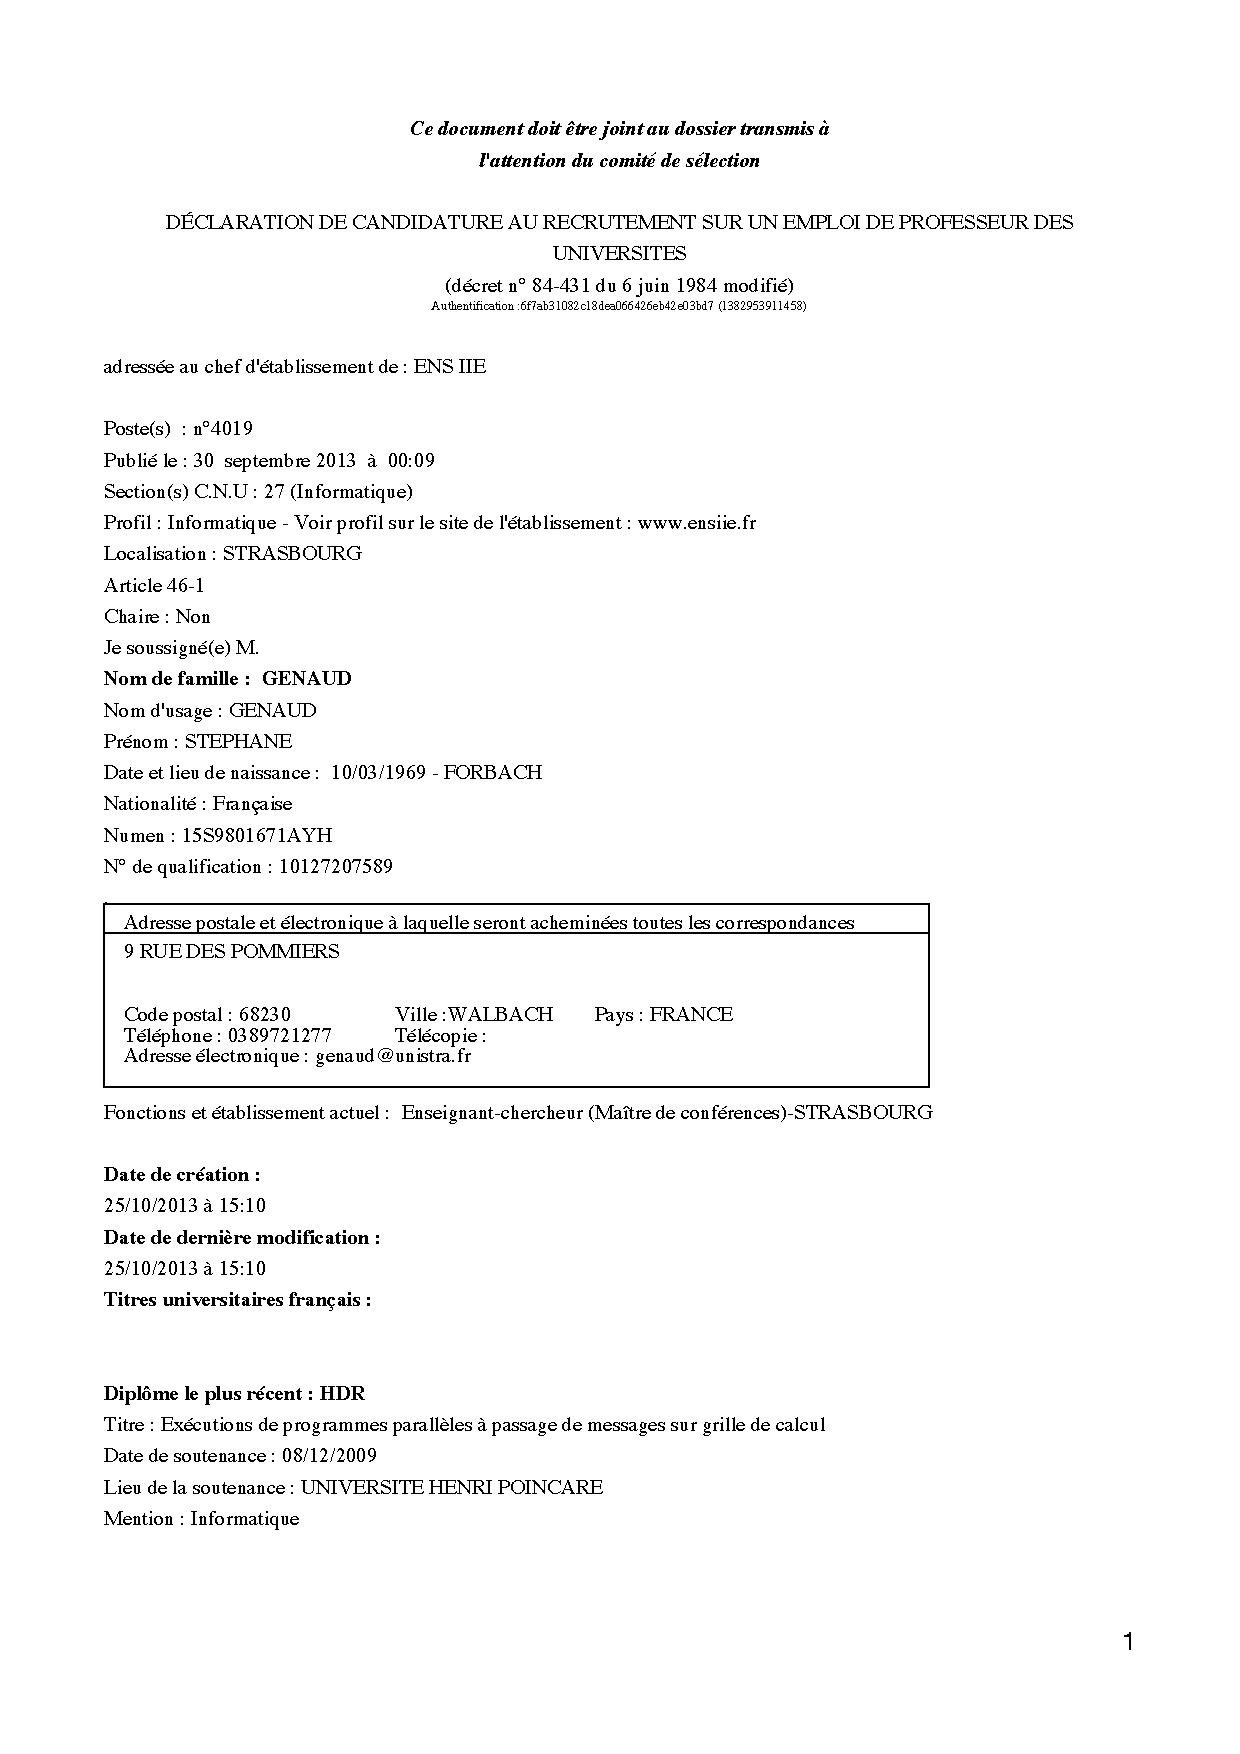
\includepdf[pages=1-2]{fiche_candidature_pr4019.pdf}
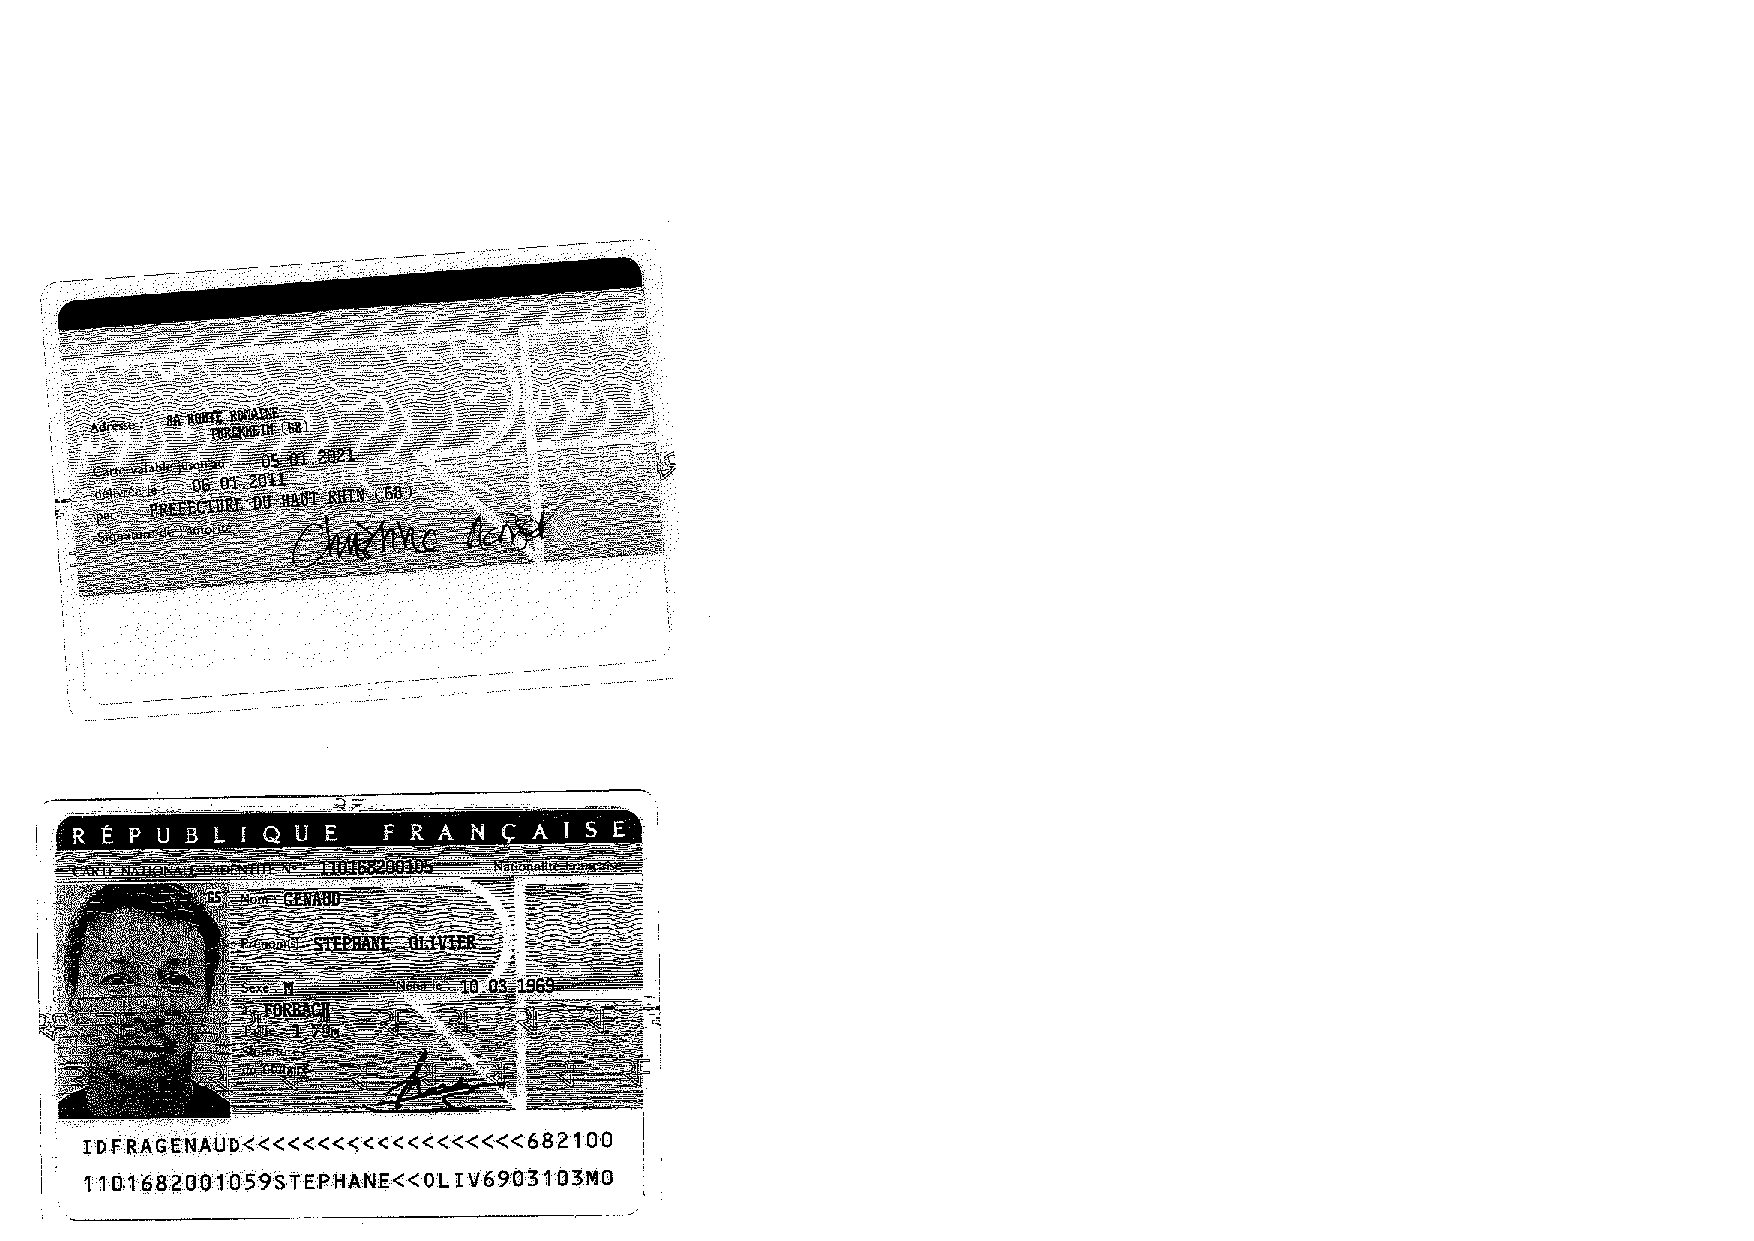
\includepdf[pages=1]{genaud_id.pdf}
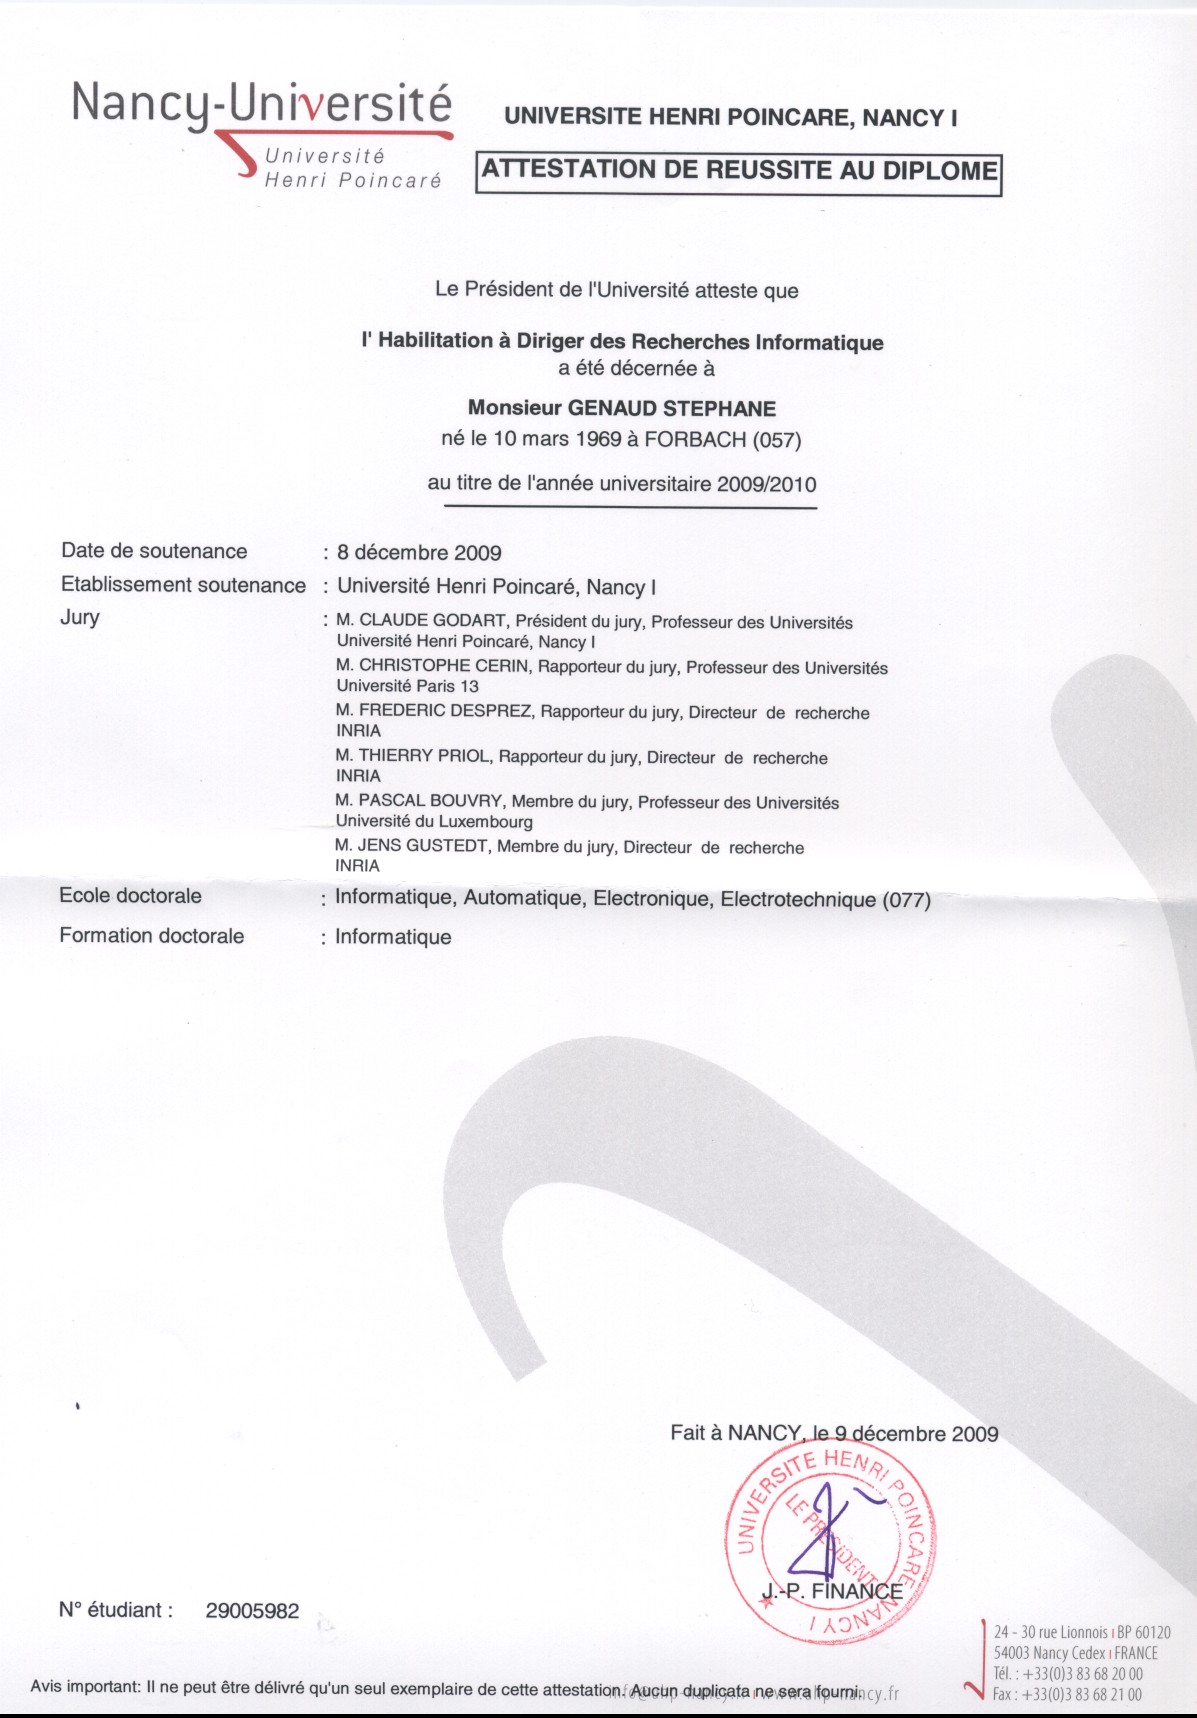
\includegraphics[height=.98\textheight]{attestation_hdr_steph.jpg}

\includepdf[pages=1]{rapport_soutenance.pdf}
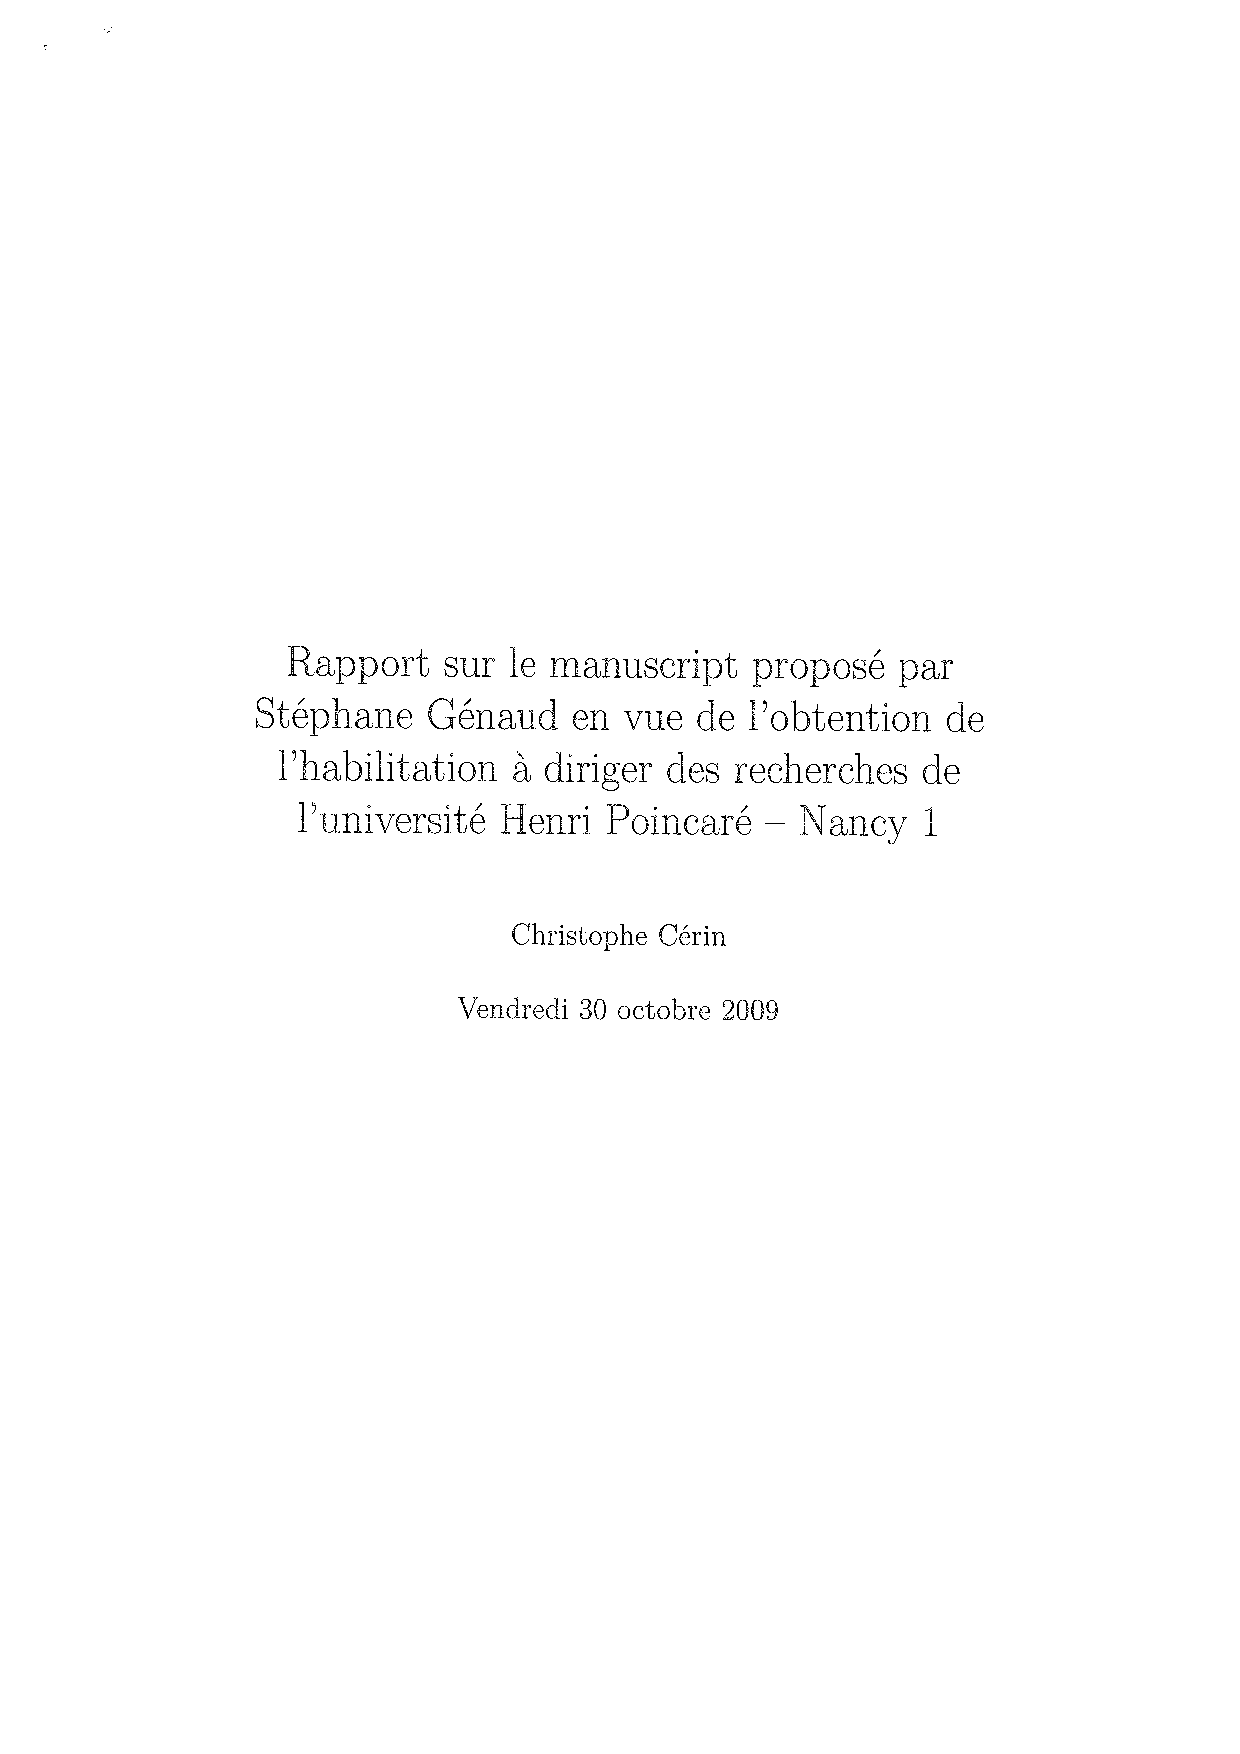
\includepdf[pages=1-5]{rapport_Cerin.pdf}
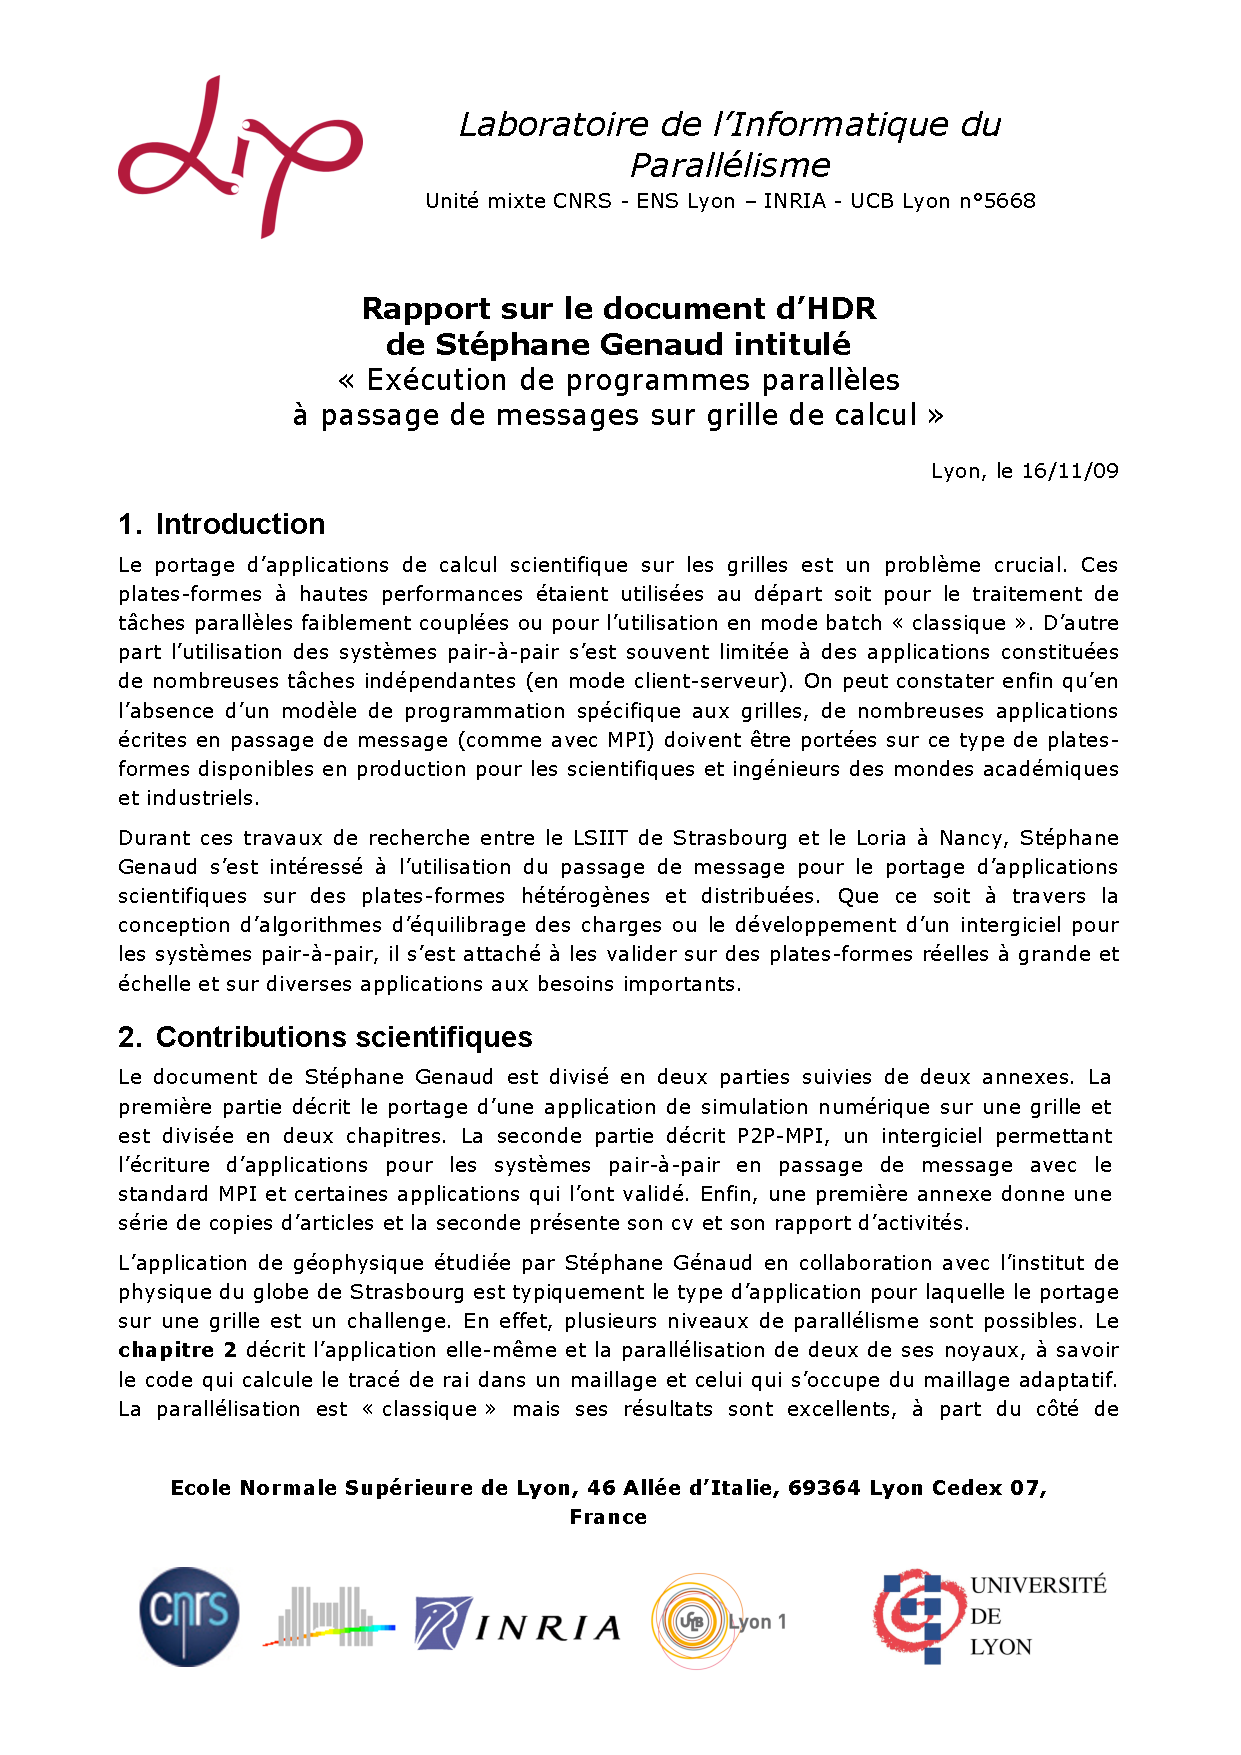
\includepdf[pages=1-2]{rapport_Desprez.pdf}
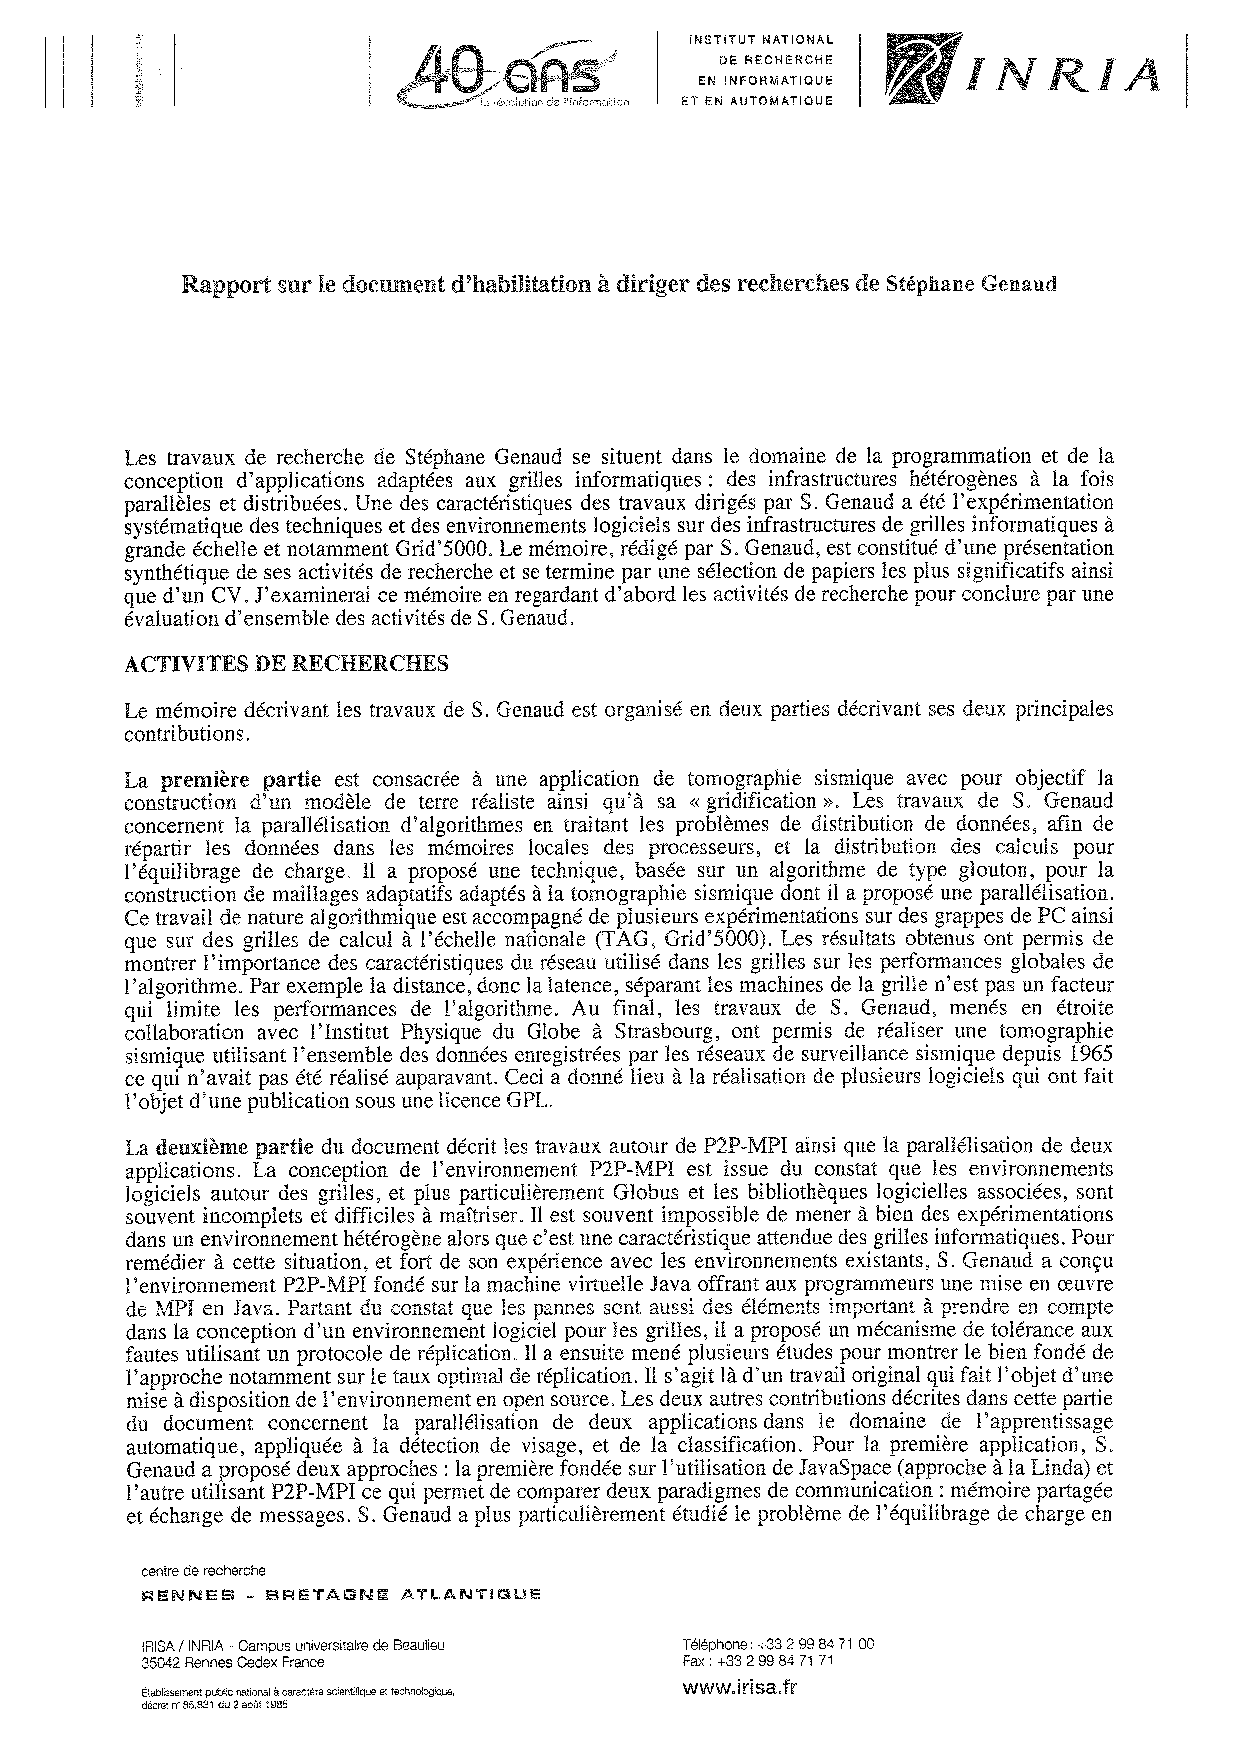
\includepdf[pages=1-2]{rapport_Priol.pdf}
%
\includepdf[pages=1]{reco_babak.pdf}
%
\includepdf[pages=1-2]{reco_jens.pdf}

%----------------------------- A R T I C L E S -------------------------------------------------------
\section{Copies d'articles}


\vspace{1cm}
Je joint ci-après six copies d'article. Ils sont classés dans un ordre chronologique inverse:

\vspace{1cm}

\begin{enumerate}
\item Article sur la simulation de programmes MPI dans le simulateur \textsc{SimGrid} (SMPI)\\
Single Node On-Line Simulation of MPI Applications with SMPI.\\
Pierre-Nicolas Clauss, Mark Stillwell, Stéphane Genaud, Fr\'ed\'eric Suter,\\
{\em 25th IEEE International Parallel \& Distributed Processing Symposium (IPDPS 2011)}, 
IEEE Computer Society Press, mai 2011.\\

\item Article sur les stratégies d'allocation de machines virtuelles dans les clouds publics IaaS.\\
Cost-wait Trade-offs in Client-side Resource Provisioning with Elastic Clouds.\\
Stéphane Genaud et Julien Gossa,\\
{\em 4th IEEE International Conference on Cloud Computing (CLOUD 2011)}, juillet 2011.\\


\item Article sur la tolérance aux pannes et la détection de pannes en P2P-MPI.\\ 
Fault-Management in P2P-MPI.\\
Stéphane Genaud, Emmanuel Jeannot et Choopan Rattanapoka.\\
{\em International Journal of Parallel Programming}, Springer, 37(5):433--461, août 2009.\\


\item Article sur la parallélisation d'une méthode de clustering avec P2P-MPI.\\
Exploitation of a parallel clustering algorithm on commodity hardware with P2P-MPI.\\
Stéphane Genaud, Pierre Gançarski, Guillaume Latu, Alexandre Blansché, Choopan Rattanapoka et Damien Vouriot.\\
{\em The Journal of SuperComputing}, Springer, 43(1):21--41, jan. 2008.\\


\item Article sur la conception de P2P-MPI\\
P2P-MPI: A Peer-to-Peer Framework for Robust Execution of Message Passing Parallel Programs on Grids.
Stéphane Genaud et Choopan Rattanapoka.\\
{\em Journal of Grid Computing}, Springer, 5(1):27--42, mai 2007.\\


\item Article sur l'équilibrage de charge.\\
Load-balancing scatter operations for Grid computing.\\
Stéphane Genaud, Arnaud Giersch, et Frédéric Vivien.\\
{\em Parallel Computing}, Elsevier, 30(8):923--946, août 2004.\\


%\item Article sur la parallélisation du tracé de rai de l'application de géophysique.\\
%Seismic ray-tracing and Earth mesh modeling on various parallel architectures.\\
%Marc Grunberg, \textbf{Stéphane Genaud} et Catherine Mongenet.\\
%{\em The Journal of Supercomputing}, Kluwer, 29(1):27--44, juillet 2004.\\
\end{enumerate}


\includepdf[pages=1-55,angle=90]{../../../../text/hdr/mypapers/papers-2pp.pdf}

% MIND LOCATION of end document



%\includepdf[pages=1-18]{../../../../myhdr/mypapers/Seismic-raytracing_JSC04.pdf}
%\includepdf[pages=1-8]{../mypapers/Mesh_coarsening_SBAC-PAD-04.pdf}
\includepdf[pages=1-24]{../../../../text/hdr/mypapers/Load-bal-scatter_ParCo04.pdf}
\includepdf[pages=1-16]{../../../../text/hdr/mypapers/P2P-MPI_joGC2007.pdf}
\includepdf[pages=1-21]{../../../../text/hdr/mypapers/Parallel-clustering-P2PMPI_JSC08.pdf}
\includepdf[pages=1-28]{../../../../text/hdr/mypapers/P2P-MPI-fault_management-IJPP.pdf}
\includepdf[pages=1-8]{../../../../text/hdr/mypapers/cloud-11.pdf}
\includepdf[pages=1-12]{../../../../text/hdr/mypapers/IPDPS-11.pdf}






\end{document}
